\documentclass[a4paper,
fontsize=11pt,
%headings=small,
oneside,
numbers=noperiodatend,
parskip=half-,
bibliography=totoc,
final
]{scrartcl}

\usepackage[babel]{csquotes}
\usepackage{synttree}
\usepackage{graphicx}
\setkeys{Gin}{width=.4\textwidth} %default pics size

\usepackage{subcaption}

\graphicspath{{./plots/}}
\usepackage[ngerman]{babel}
\usepackage[T1]{fontenc}
%\usepackage{amsmath}
\usepackage[utf8x]{inputenc}
\usepackage [hyphens]{url}
\usepackage{booktabs} 
\usepackage[left=2.4cm,right=2.4cm,top=2.3cm,bottom=2cm,includeheadfoot]{geometry}
\usepackage[labelformat=empty]{caption} % option 'labelformat=empty]' to surpress adding "Abbildung 1:" or "Figure 1" before each caption / use parameter '\captionsetup{labelformat=empty}' instead to change this for just one caption
\usepackage{eurosym}
\usepackage{multirow}
\usepackage[ngerman]{varioref}
\setcapindent{1em}
\renewcommand{\labelitemi}{--}
\usepackage{paralist}
\usepackage{pdfpages}
\usepackage{lscape}
\usepackage{float}
\usepackage{acronym}
\usepackage{eurosym}
\usepackage{longtable,lscape}
\usepackage{mathpazo}
\usepackage[normalem]{ulem} %emphasize weiterhin kursiv
\usepackage[flushmargin,ragged]{footmisc} % left align footnote
\usepackage{ccicons} 
\setcapindent{0pt} % no indentation in captions
\usepackage{xurl} % Breaks URLs

%%%% fancy LIBREAS URL color 
\usepackage{xcolor}
\definecolor{libreas}{RGB}{112,0,0}

\usepackage{listings}

\urlstyle{same}  % don't use monospace font for urls

\usepackage[fleqn]{amsmath}

%adjust fontsize for part

\usepackage{sectsty}
\partfont{\large}

%Das BibTeX-Zeichen mit \BibTeX setzen:
\def\symbol#1{\char #1\relax}
\def\bsl{{\tt\symbol{'134}}}
\def\BibTeX{{\rm B\kern-.05em{\sc i\kern-.025em b}\kern-.08em
    T\kern-.1667em\lower.7ex\hbox{E}\kern-.125emX}}

\usepackage{fancyhdr}
\fancyhf{}
\pagestyle{fancyplain}
\fancyhead[R]{\thepage}

% make sure bookmarks are created eventough sections are not numbered!
% uncommend if sections are numbered (bookmarks created by default)
\makeatletter
\renewcommand\@seccntformat[1]{}
\makeatother

% typo setup
\clubpenalty = 10000
\widowpenalty = 10000
\displaywidowpenalty = 10000

\usepackage{hyperxmp}
\usepackage[colorlinks, linkcolor=black,citecolor=black, urlcolor=libreas,
breaklinks= true,bookmarks=true,bookmarksopen=true]{hyperref}
\usepackage{breakurl}

%meta
%meta

\fancyhead[L]{M. Roth et al.\\ %author
LIBREAS. Library Ideas, 45 (2024). % journal, issue, volume.
\href{https://doi.org/10.18452/...}{\color{black}https://doi.org/10.18452/...}
{}} % doi 
\fancyhead[R]{\thepage} %page number
\fancyfoot[L] {\ccLogo \ccAttribution\ \href{https://creativecommons.org/licenses/by/4.0/}{\color{black}Creative Commons BY 4.0}}  %licence
\fancyfoot[R] {ISSN: 1860-7950}

\title{\LARGE{Die Bibliothek von Basel. Unendliche Klänge und eine neue Heimat}}% title
\author{Michel Roth, Felicitas Erb, Anna Alexay, \\ Oleksandra Katsalap, Oliver Rutz} % author

\setcounter{page}{1}

\hypersetup{%
      pdftitle={Die Bibliothek von Basel. Unendliche Klänge und eine neue Heimat},
     pdfauthor={Michel Roth, Felicitas Erb, Anna Alexay, Oleksandra Katsalap, Oliver Rutz},
      pdfcopyright={CC BY 4.0 International},
      pdfsubject={LIBREAS. Library Ideas, 45 (2024).},
      pdfkeywords={Vera Oeri Bibliothek, Basel, Klang, Soundkarte},
      pdflicenseurl={https://creativecommons.org/licenses/by/4.0/},
      pdfurl={https://doi.org/10.18452/...},
      pdfdoi={10.18452/...},
      pdflang={de},
      pdfmetalang={de}
     }



\date{}
\begin{document}

\maketitle
\thispagestyle{fancyplain} 

%abstracts

%body
Die Bibliothek von Babel, beschrieben von Jorge Luis Borges, ist ein
stiller Ort. Jedenfalls widmet sich die gleichnamige Erzählung nur ihrer
visuellen Erscheinung: Selbst Bücherverbrennungen und
Selbstmordndcloude, die sich laut Borges in diesem papierenen Universum
ereignen, scheinen lautlos zu geschehen. Zwar wird behauptet, dass diese
unendliche Bibliothek alle kombinatorisch möglichen Bücher enthalte,
doch die Erzählung verweist vor allem auf sich selbst, auf fiktionale
Literatur und Literaturwissenschaft. Bücher über Musik finden z. B.
keine Erwähnung -- vielleicht weil sie sich nicht einfach einreihen
lassen als weitere fantastische Konstellation von 25 Schriftzeichen,
sondern ebenso Notenbeispiele, ergänzende Tonträger und Porträts von
ernst blickenden Komponisten erfordern.

Die Bibliothek von Basel, die Vera Oeri Bibliothek der Musik-Akademie
Basel\footnote{\url{https://www.musik-akademie.ch/bibliothek/de.html}},
stellt als grösste Musikaliensammlung der Schweiz also Borges'
Bibliothek spielend in den Schatten: Dieses Universum ist wirklich
unendlich, nicht als Magazin oder Bibliothekskatalog, sondern in den
unendlichen Möglichkeiten, diese Noten, Tonträger, Datenbanken und
Media-Kits zu nutzen, zu interpretieren und mit anderen zu teilen.
Mitten in der Stadt Basel ist die Bibliothek zwar ein Raum der Stille,
doch gefüllt mit Musik und nicht ruhig: In der \enquote{Musikbox}
spielen Kinder Musikspiele, im Co-Working-Space werden
Musikvermittlungsprojekte diskutiert oder Eigenkompositionen in eine
Notationssoftware getippt und Musik aus allen Zeiten wird im Kopierraum
geräuschvoll durch die Maschine gezogen, um sie an einem anderen Ort zu
spielen, aber auch im Lesesaal zu studieren, also sich innerlich
vorzustellen.

\begin{figure}
\centering
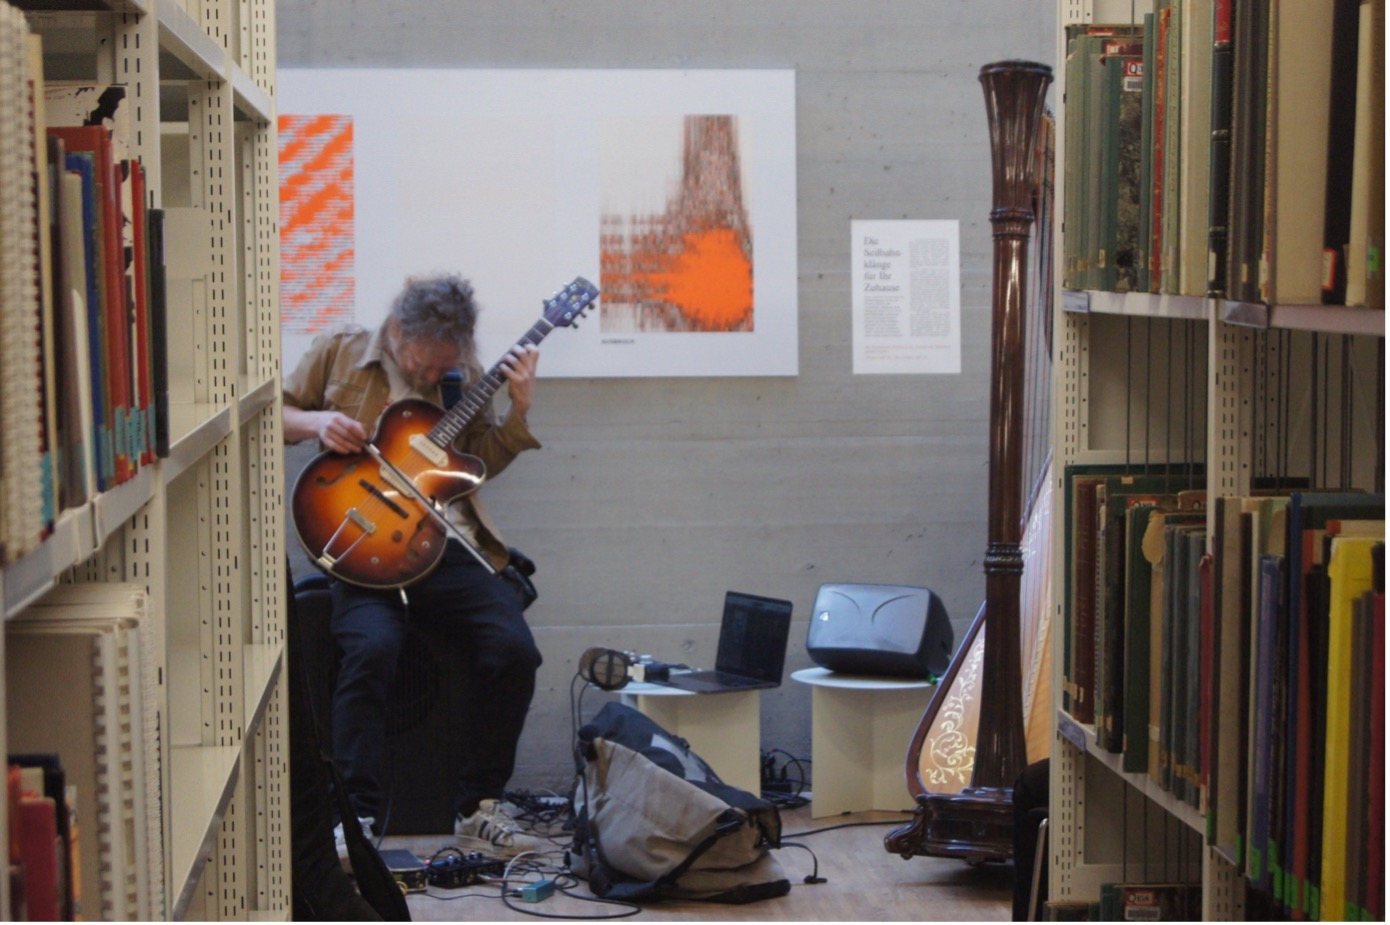
\includegraphics{img/Abb1.jpg}
\caption{Abbildung 1: Mikael Szafirowski, Student am Sonic Space Basel
der Hochschule für Musik Basel, improvisiert in der Vera Oeri Bibliothek
zu live gestreamten Klängen des Lüftungssystems und einer alpinen
Seilbahn. Foto: Christoph Moor.}
\end{figure}

\hypertarget{luftige-ohrwuxfcrmer}{%
\section{Luftige Ohrwürmer}\label{luftige-ohrwuxfcrmer}}

Wenn man alle Klänge und Ohrwürmer, die die Nutzer:innen der Vera Oeri
Bibliothek im Kopf mit sich tragen, hörbar machen könnte, das ergäbe
nicht was Borges in seiner Bibliothek als \enquote{Meilen sinnloser
Kakophonien} beschreibt, sondern eine polyphone, klangräumlich
differenzierte Mehrchörigkeit, wie sie Wim Wenders in der berühmten
Bibliotheksszene von \emph{Der Himmel über Berlin} (1987)\footnote{\url{https://www.youtube.com/watch?v=3LsUFzuTeS4}}
als \emph{Soundwalk} inszeniert: In der spektakulären Architektur der
Berliner Stabi präsentiert sich der Klang zwar als ephemer und flüchtig,
doch gerade deshalb formbar in Zeit und Raum, performativ und metamorph.

Nun ist die Hochschule für Musik Basel, unter dem selben Dach wie die
Vera Oeri Bibliothek, tatsächlich im Besitz einer potenziell unendlichen
Klangbibliothek: Seit 2020 zeichnet der Schweizer Komponist und
Musikforscher Michel Roth Eigenschwingungen von Seilbahnseilen in den
Urner Alpen auf. Diese so genannten \enquote{Singenden Seile} treten vor
allem auf, wenn die Bahn nicht fährt; die Einheimischen beobachten das
Phänomen über Stunden und Tage, nachts stört es sie manchmal, doch es
bedeutet auch etwas Vertrautes und Heimatliches und begleitet sie durch
die Jahreszeiten. Bergbauern nutzen das Singen zur lokalen
Wettervorhersage. Roths Tonarchiv\footnote{\url{http://www.ropesinging.ch}}
umfasst bereits Hunderte von Aufnahmen, wobei er ein Gerät entwickelt
hat, das Seilklänge auch live streamen und damit endlos aufzeichnen
lässt\footnote{\url{http://www.seilsender.ch}}.

\begin{figure}
\centering
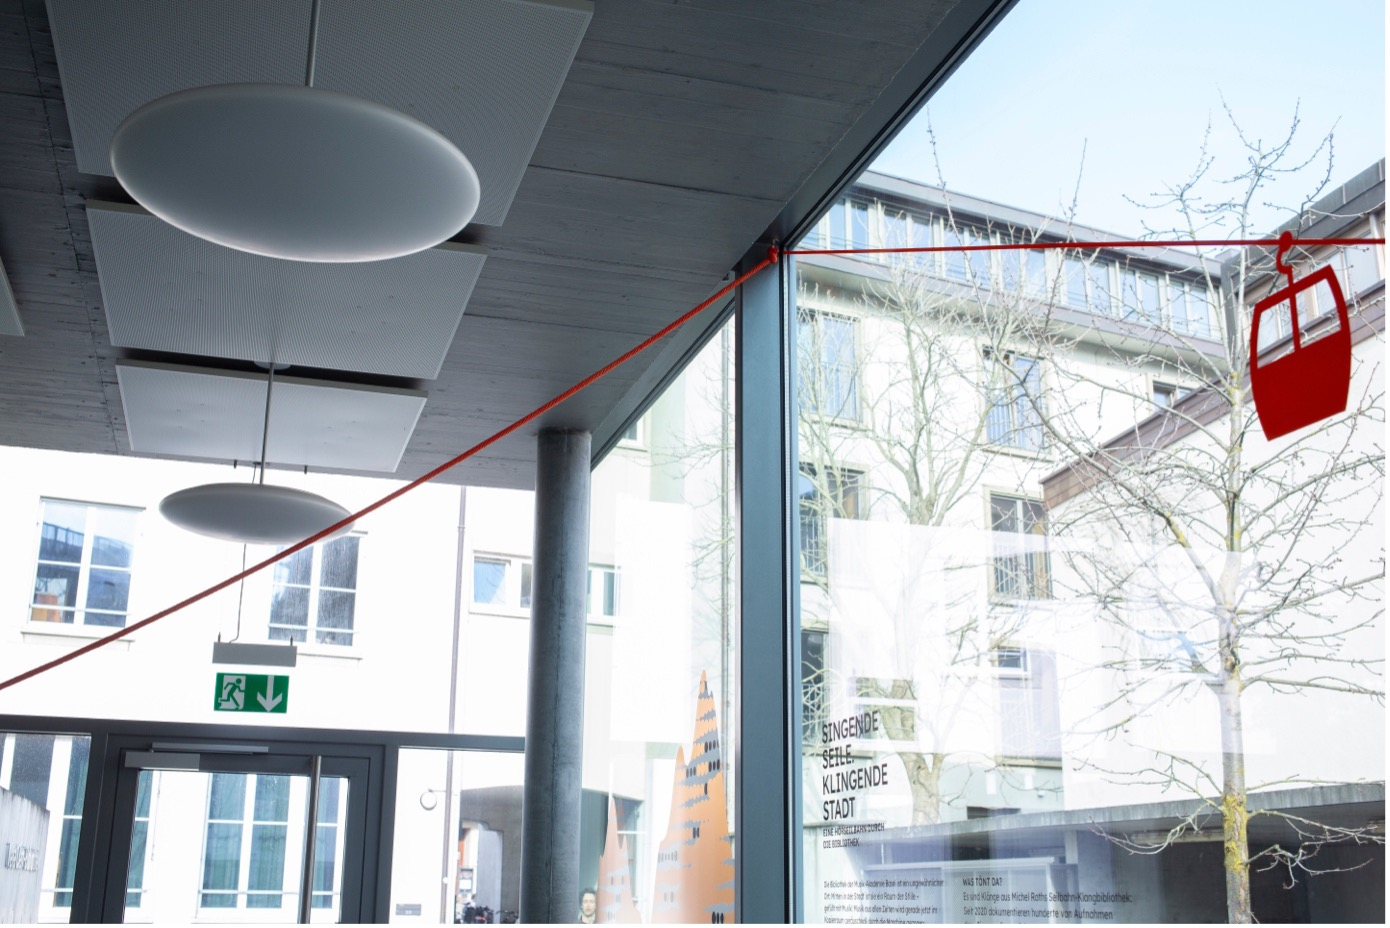
\includegraphics{img/Abb2.jpg}
\caption{Abbildung 2: Eingangsfoyer der Vera Oeri Bibliothek mit
Infotafel der Ausstellung \emph{Singende Seile. Klingende Stadt. Eine
Hörseilbahn durch die Bibliothek.} Foto: Szenografie Stauffenegger +
Partner.}
\end{figure}

\hypertarget{von-der-klangbibliothek-zum-klang-der-bibliothek}{%
\section{Von der Klangbibliothek zum Klang der
Bibliothek}\label{von-der-klangbibliothek-zum-klang-der-bibliothek}}

Dieser Klangbibliothek und dem zugehörigen Forschungsprojekt hat die
Vera Oeri Bibliothek im März 2024 eine Ausstellung mit
Begleitprogramm\footnote{\url{https://www.fhnw.ch/de/forschung-und-dienstleistungen/musik/hochschule-fuer-musik-klassik/veranstaltungen/2023-24/singende-seile-klingende-stadt}}
gewidmet, die unter dem Titel \emph{Singende Seile. Klingende Stadt}
auch den Transfer in die akustische Ökologie des urbanen Raums
thematisiert: Welche Klänge prägen unseren Alltag in der Stadt, welche
beobachten wir, geben uns Identität und Orientierung oder deuten auf
Veränderungen unserer Umwelt hin beziehungsweise werden als störend
empfunden?

\begin{figure}[h]
\centering
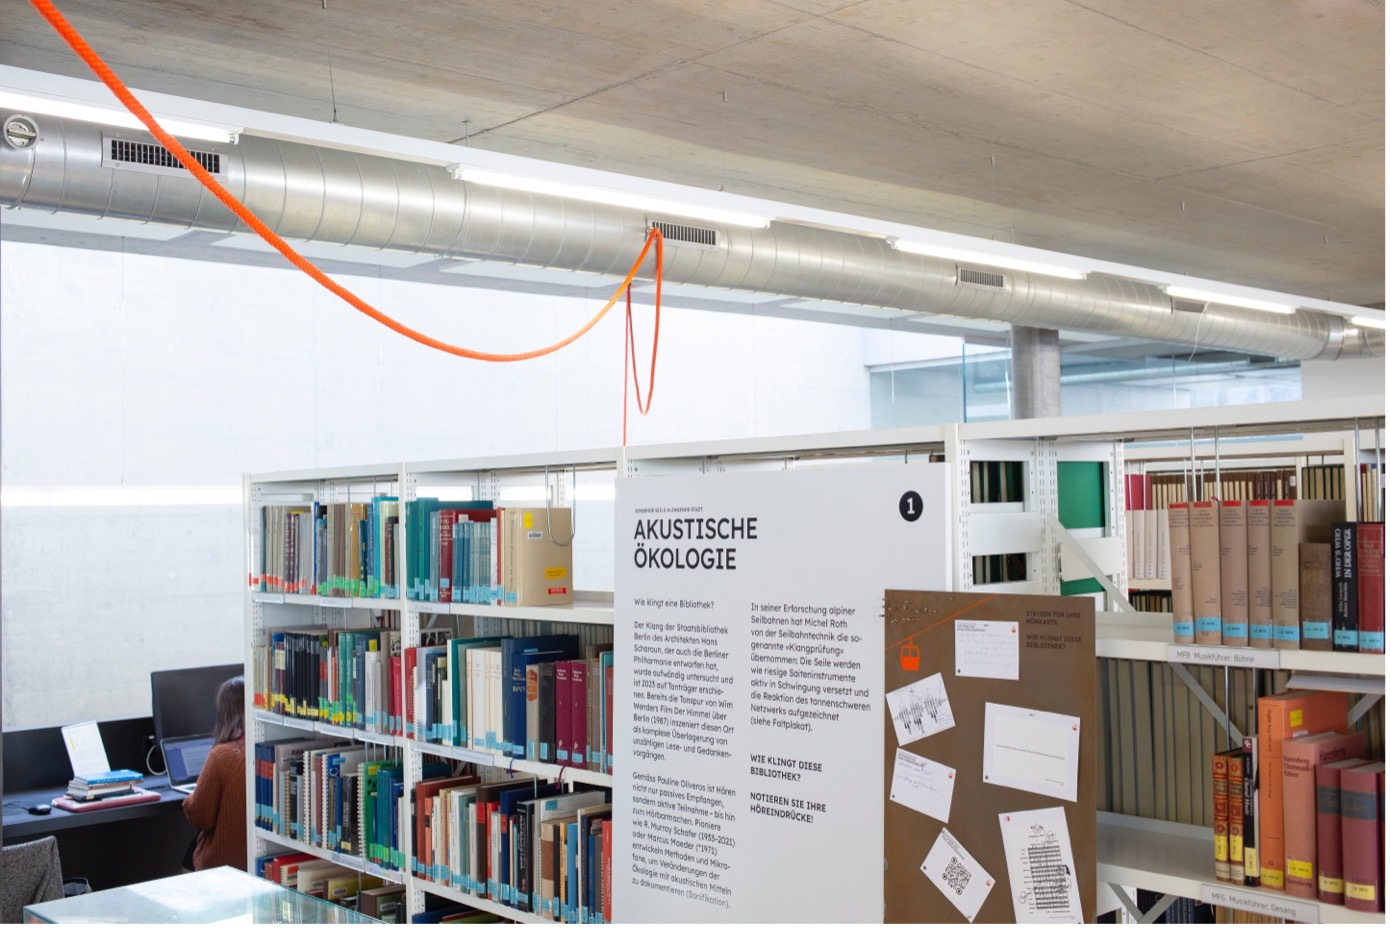
\includegraphics{img/Abb3.jpg}
\caption{Abbildung 3: Lesesaal der Vera Oeri Bibliothek mit verspannten
Seilen als visuelle Signalisation des Verlaufs der Hörseilbahn, ebenso
Tafeln mit Hintergrundinformationen und Einladung ans Publikum, über den
Klang der Bibliothek nachzudenken. Foto: Szenografie Stauffenegger +
Partner.}
\end{figure}

\begin{figure}[H]
\centering
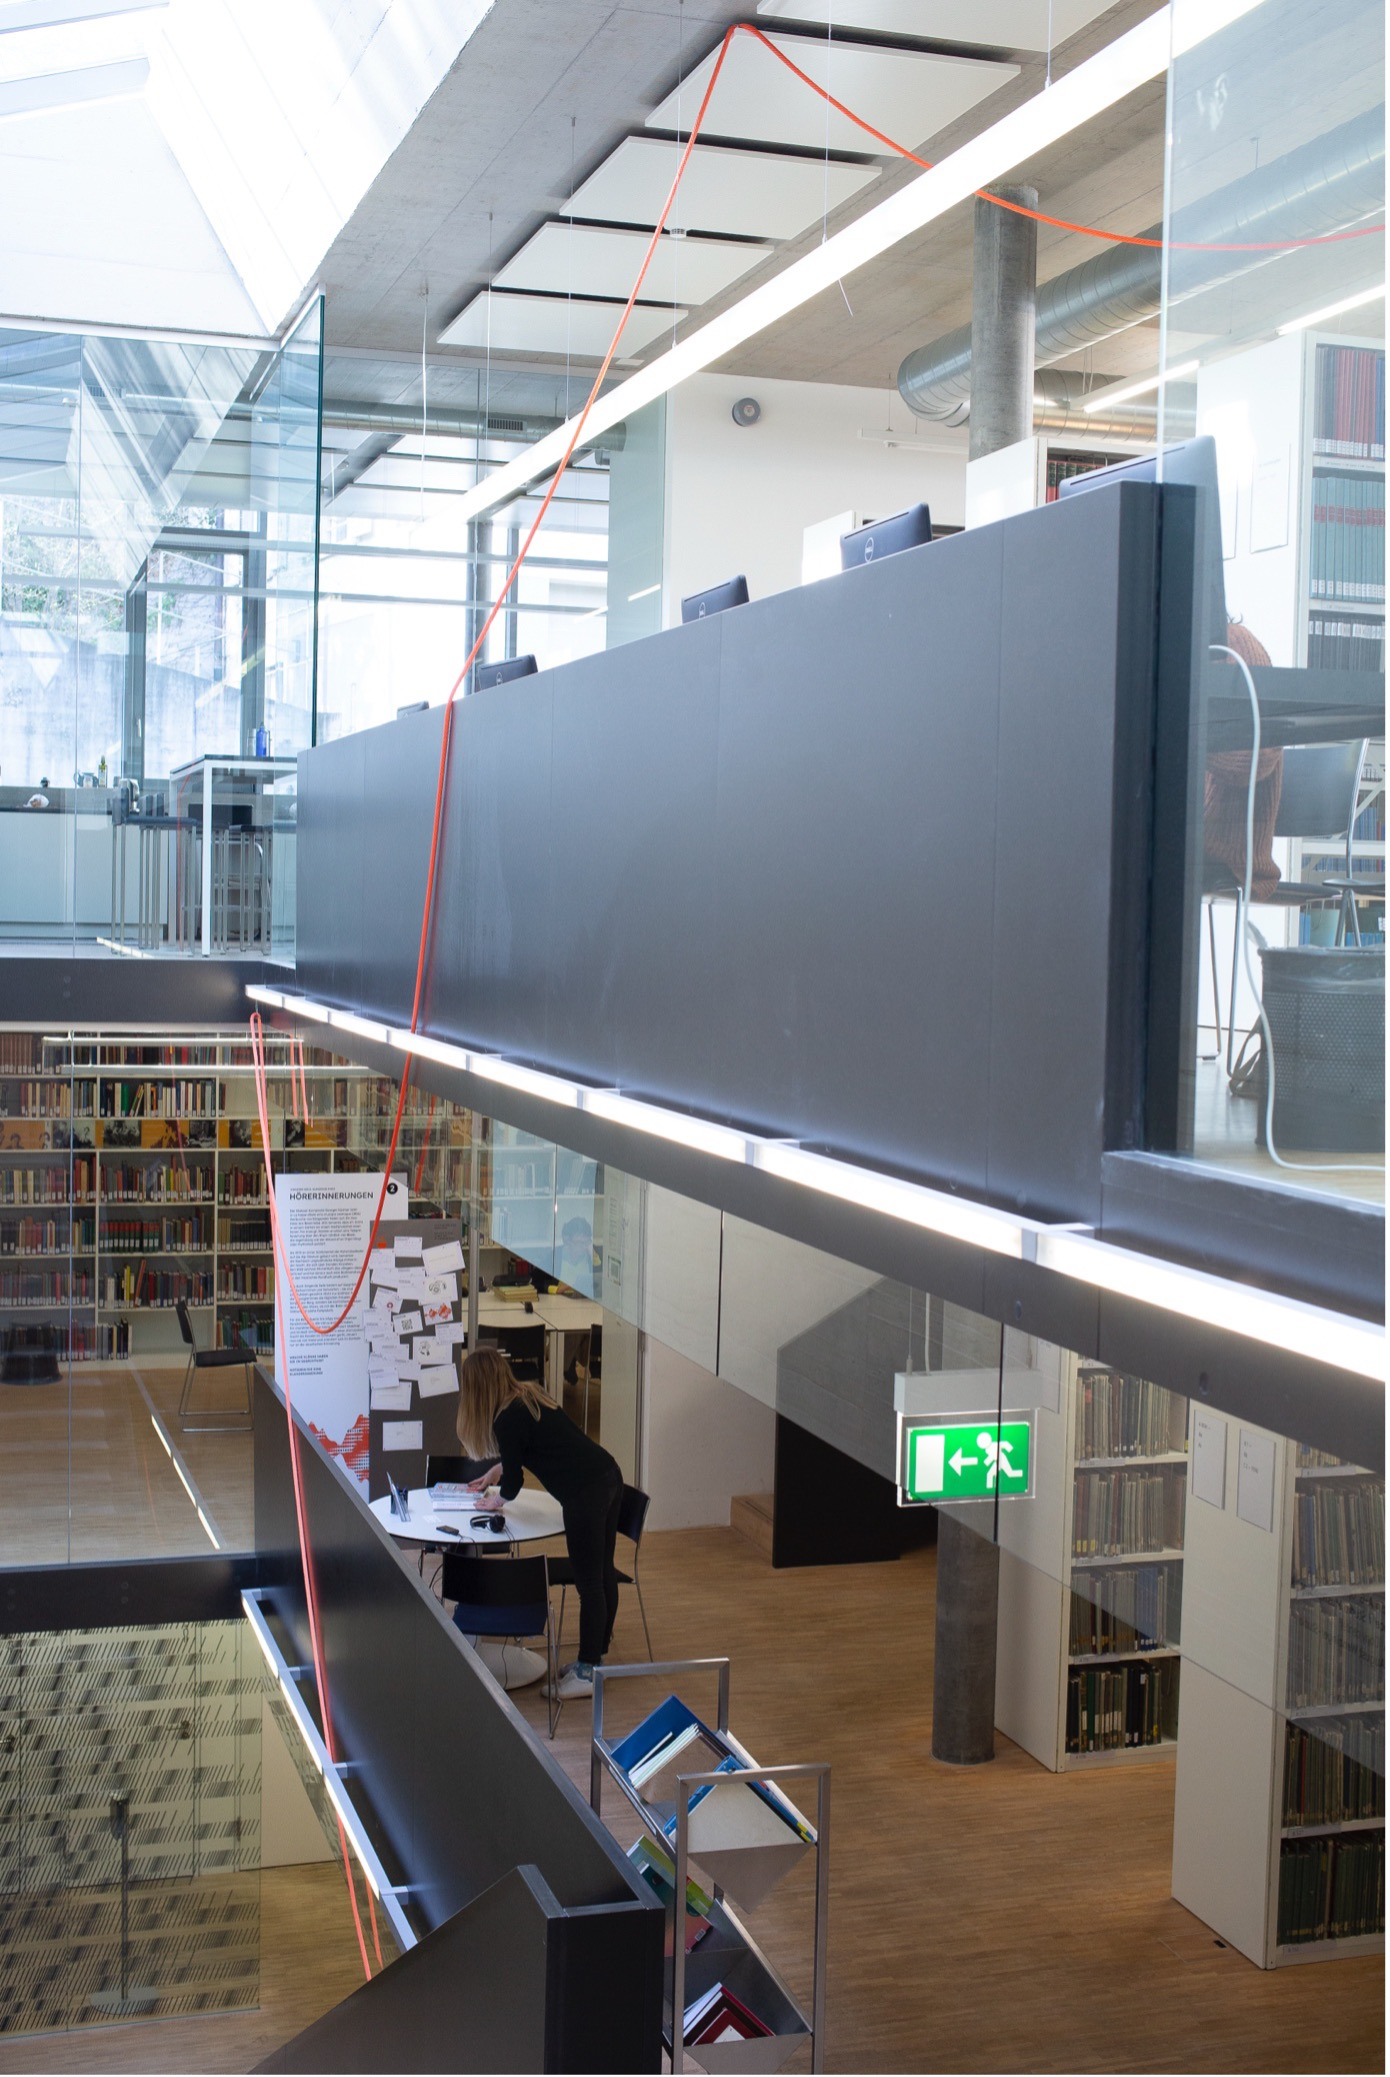
\includegraphics{img/Abb4.jpg}
\caption{Abbildung 4: Das Seil und damit die Ausstellung führt über
insgesamt vier Stockwerke quer durch die Vera Oeri Bibliothek. Foto:
Szenografie Stauffenegger + Partner.}
\end{figure}

Nebst live gestreamten Klängen aus den Alpen und Zugriff auf Michel
Roths digitale Klangbibliothek verwandelte sich die Vera Oeri Bibliothek
in eine Klangseilbahn: Szenografisch geführt von im Raum verspannten
orangen Seilen konnte man über vier Stationen und Etagen (entlang der
vier Hörachsen der amerikanischen Komponistin Pauline Oliveros) den
Klangraum der Bibliothek erkunden.

\hypertarget{huxf6rachse}{%
\subsection{1. Hörachse}\label{huxf6rachse}}

Das Publikum wurde mit Postkarten zu eigenen Hörexperimenten angeleitet,
zum Beispiel:

\begin{figure}[h]
\centering
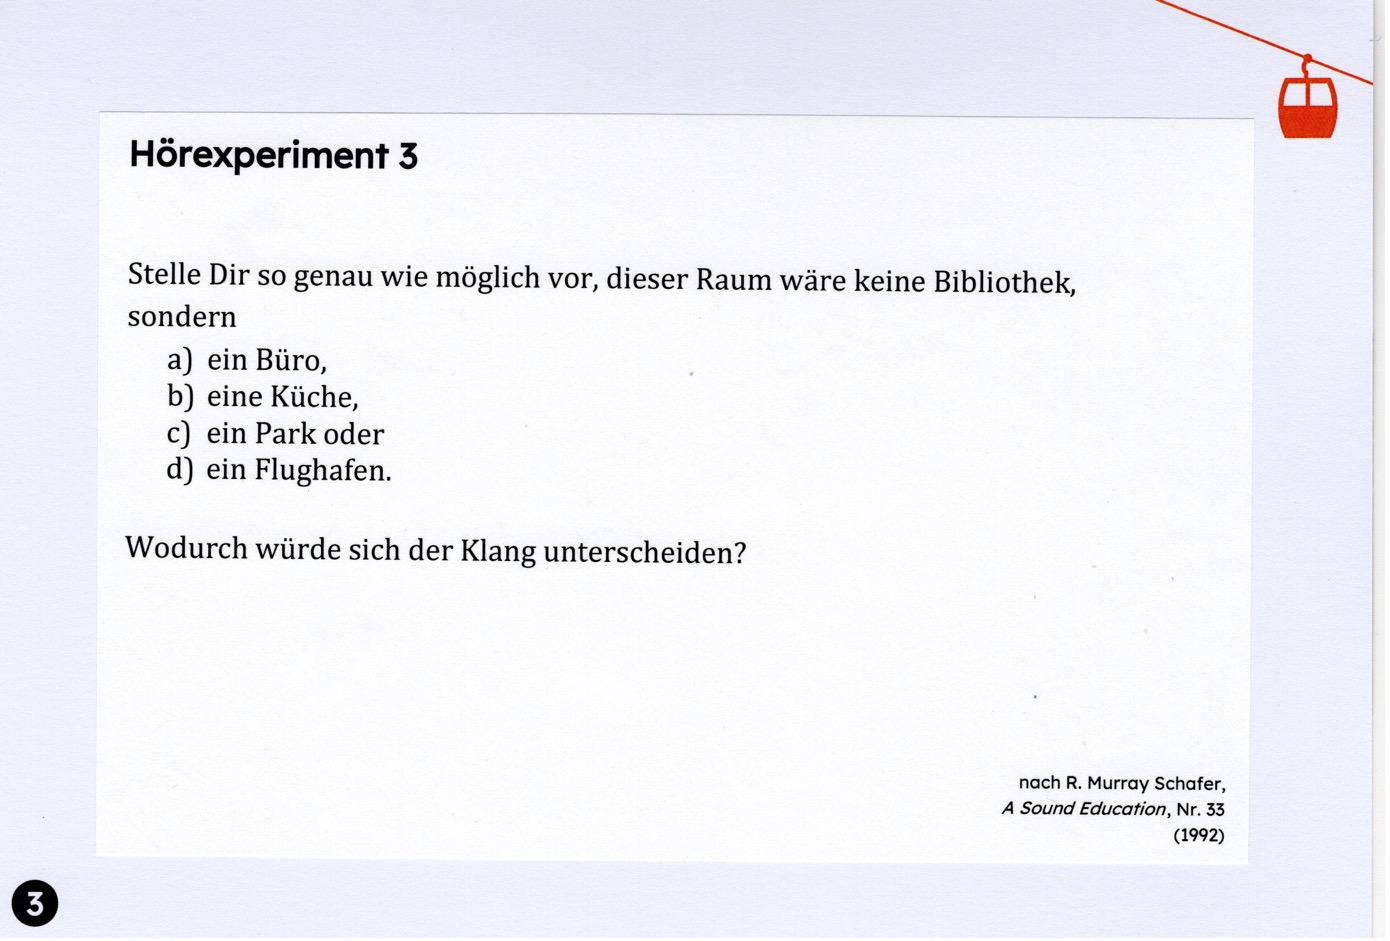
\includegraphics{img/Abb5.jpg}
\caption{Abbildung 5: Eine von mehreren in der Bibliothek verteilten
Postkarten mit Hörexperimenten. Viele entstammen Büchern und anderen
Medien, die Teil des Bestands der Vera Oeri Bibliothek sind.}
\end{figure}

\hypertarget{huxf6rachse-1}{%
\subsection{2. Hörachse}\label{huxf6rachse-1}}

Die Besuchenden wurden gebeten, den Klang der Bibliothek auf
bereitgelegten Postkarten zu beschreiben:


\begin{figure}[H]
    \centering
    \begin{minipage}[b]{0.45\textwidth}
        \centering
        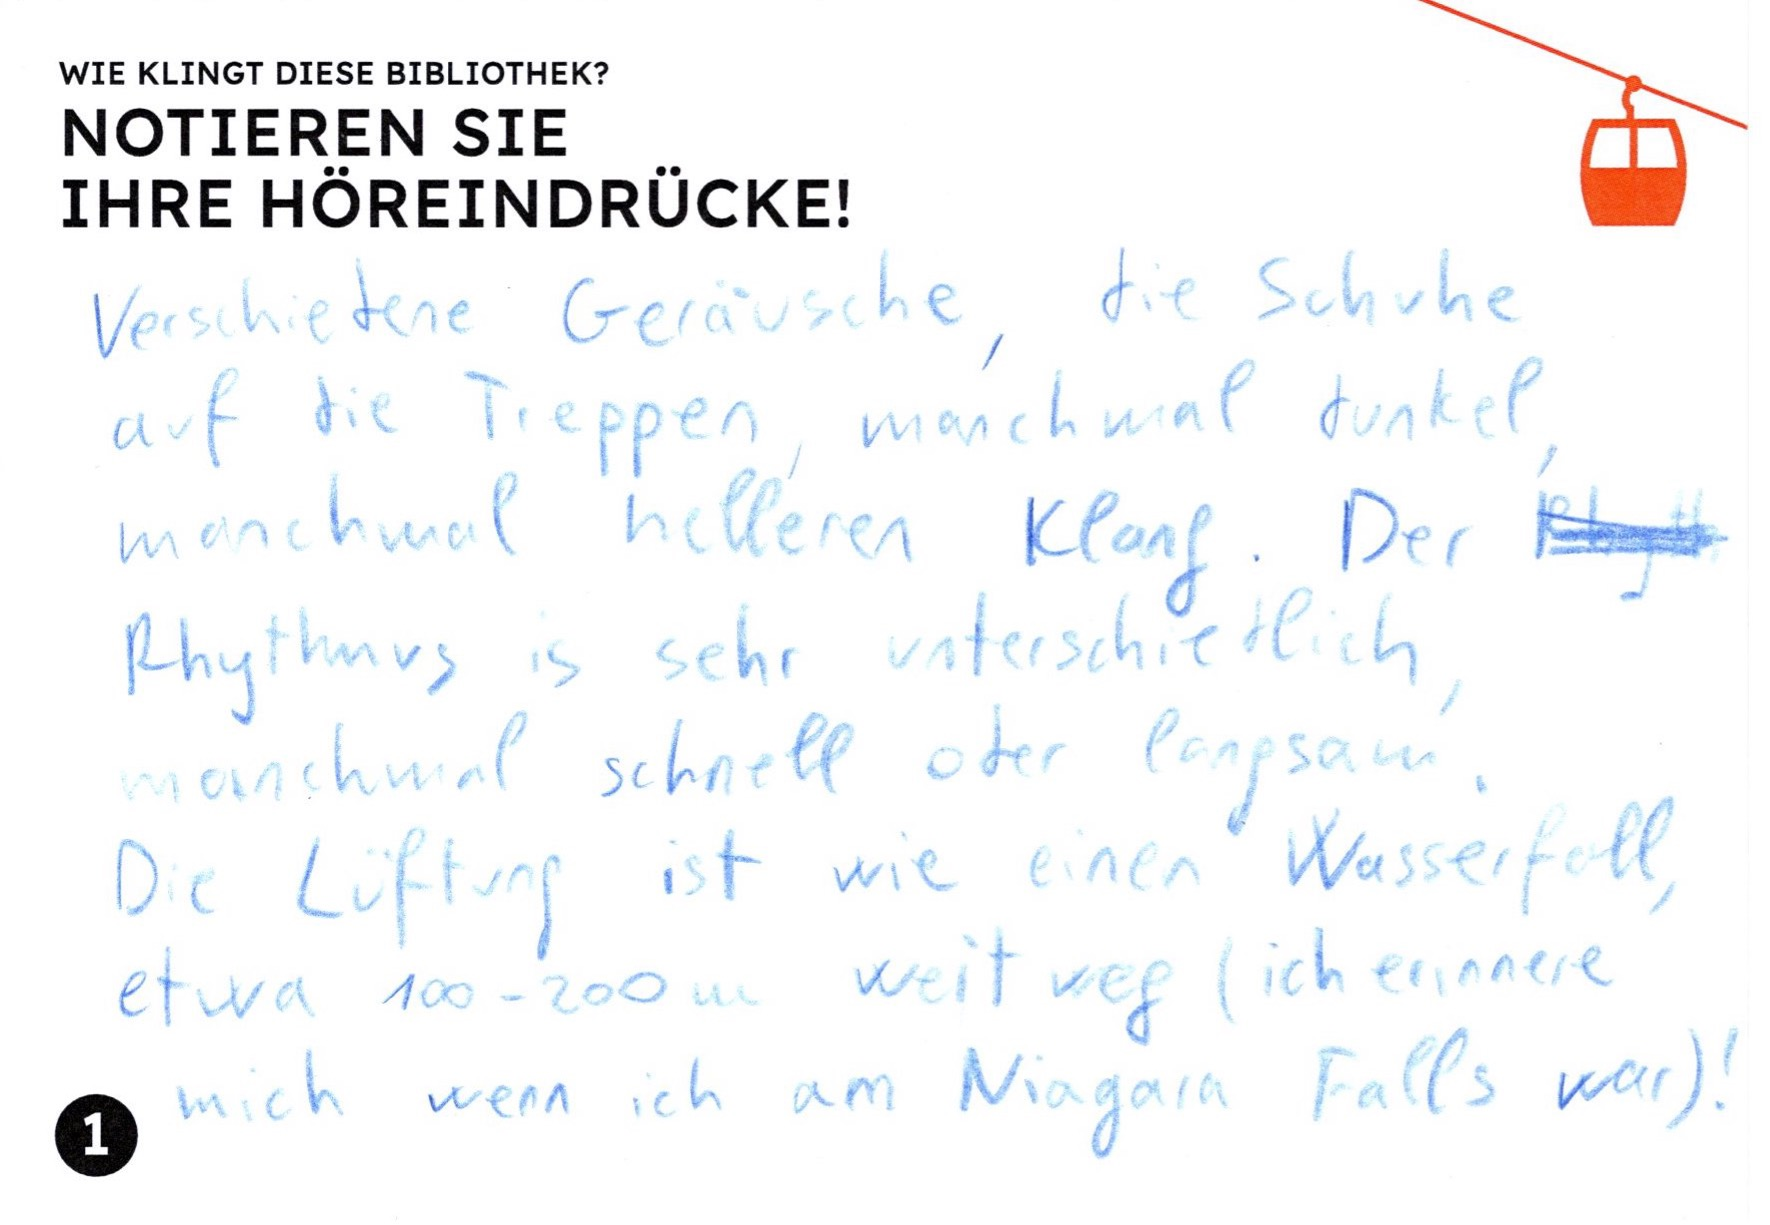
\includegraphics[width=\textwidth]{img/Abb6.jpg}
    \end{minipage}
    \begin{minipage}[b]{0.45\textwidth}
        \centering
        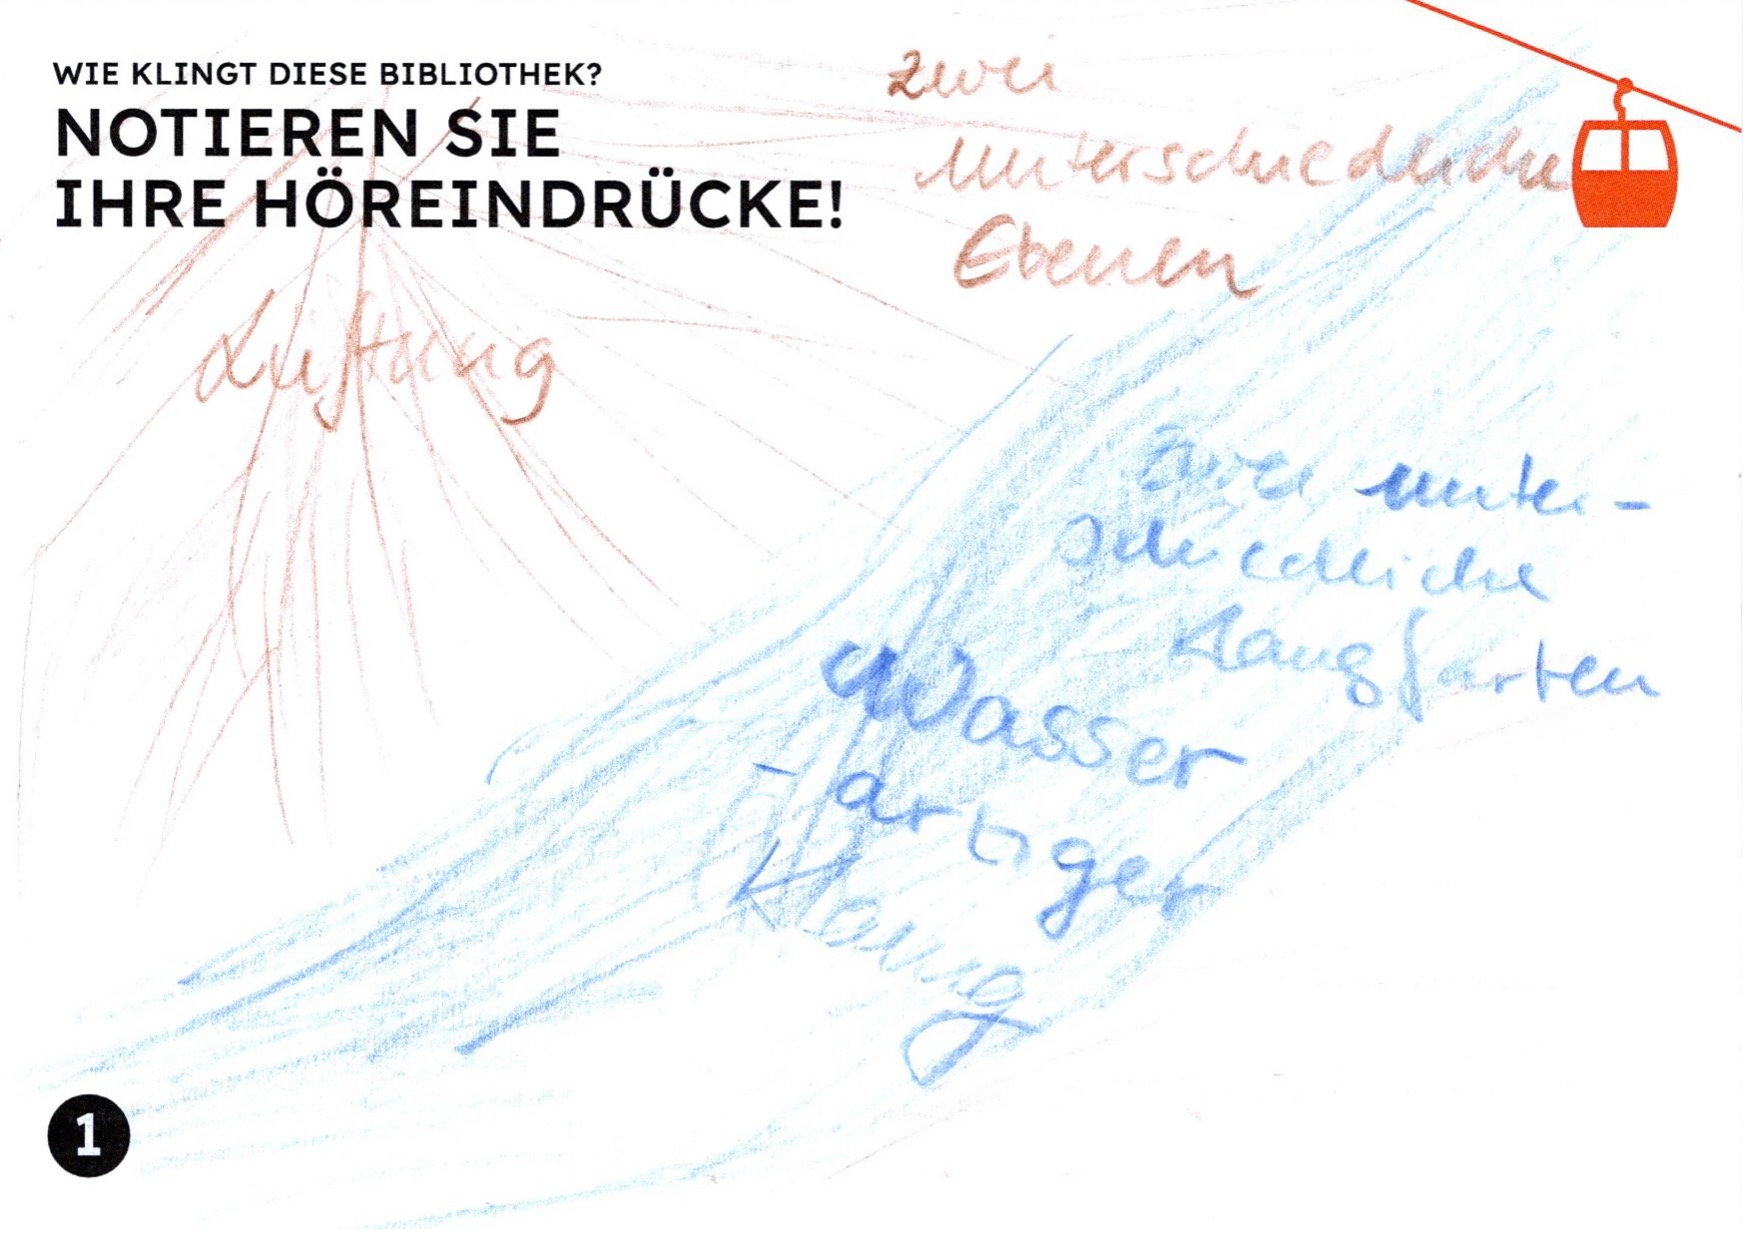
\includegraphics[width=\textwidth]{img/Abb7.jpg}
    \end{minipage}
    
    \vspace{0.5cm}
    
    \begin{minipage}[b]{0.45\textwidth}
        \centering
        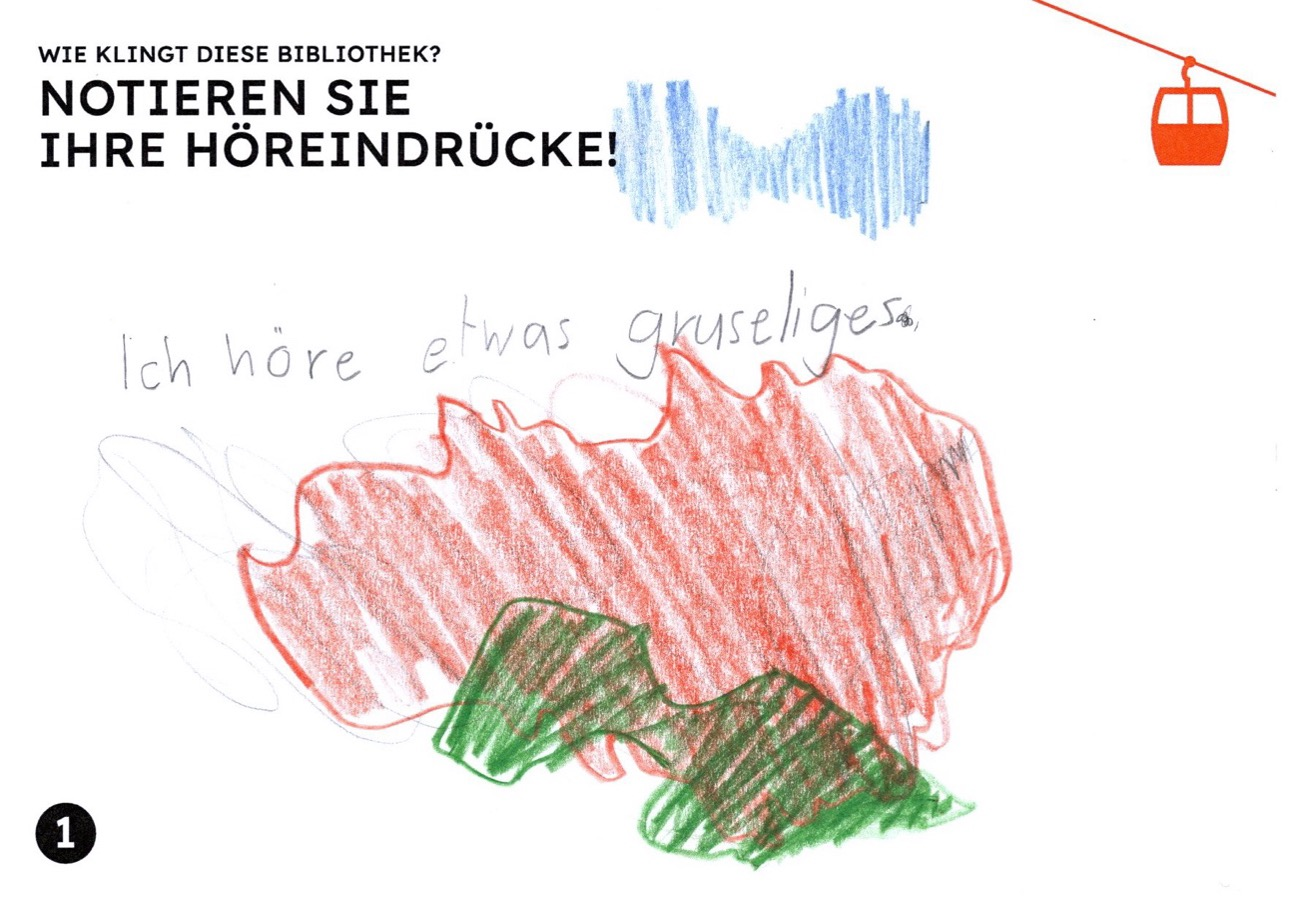
\includegraphics[width=\textwidth]{img/Abb8.jpg}
    \end{minipage}
    \begin{minipage}[b]{0.45\textwidth}
        \centering
        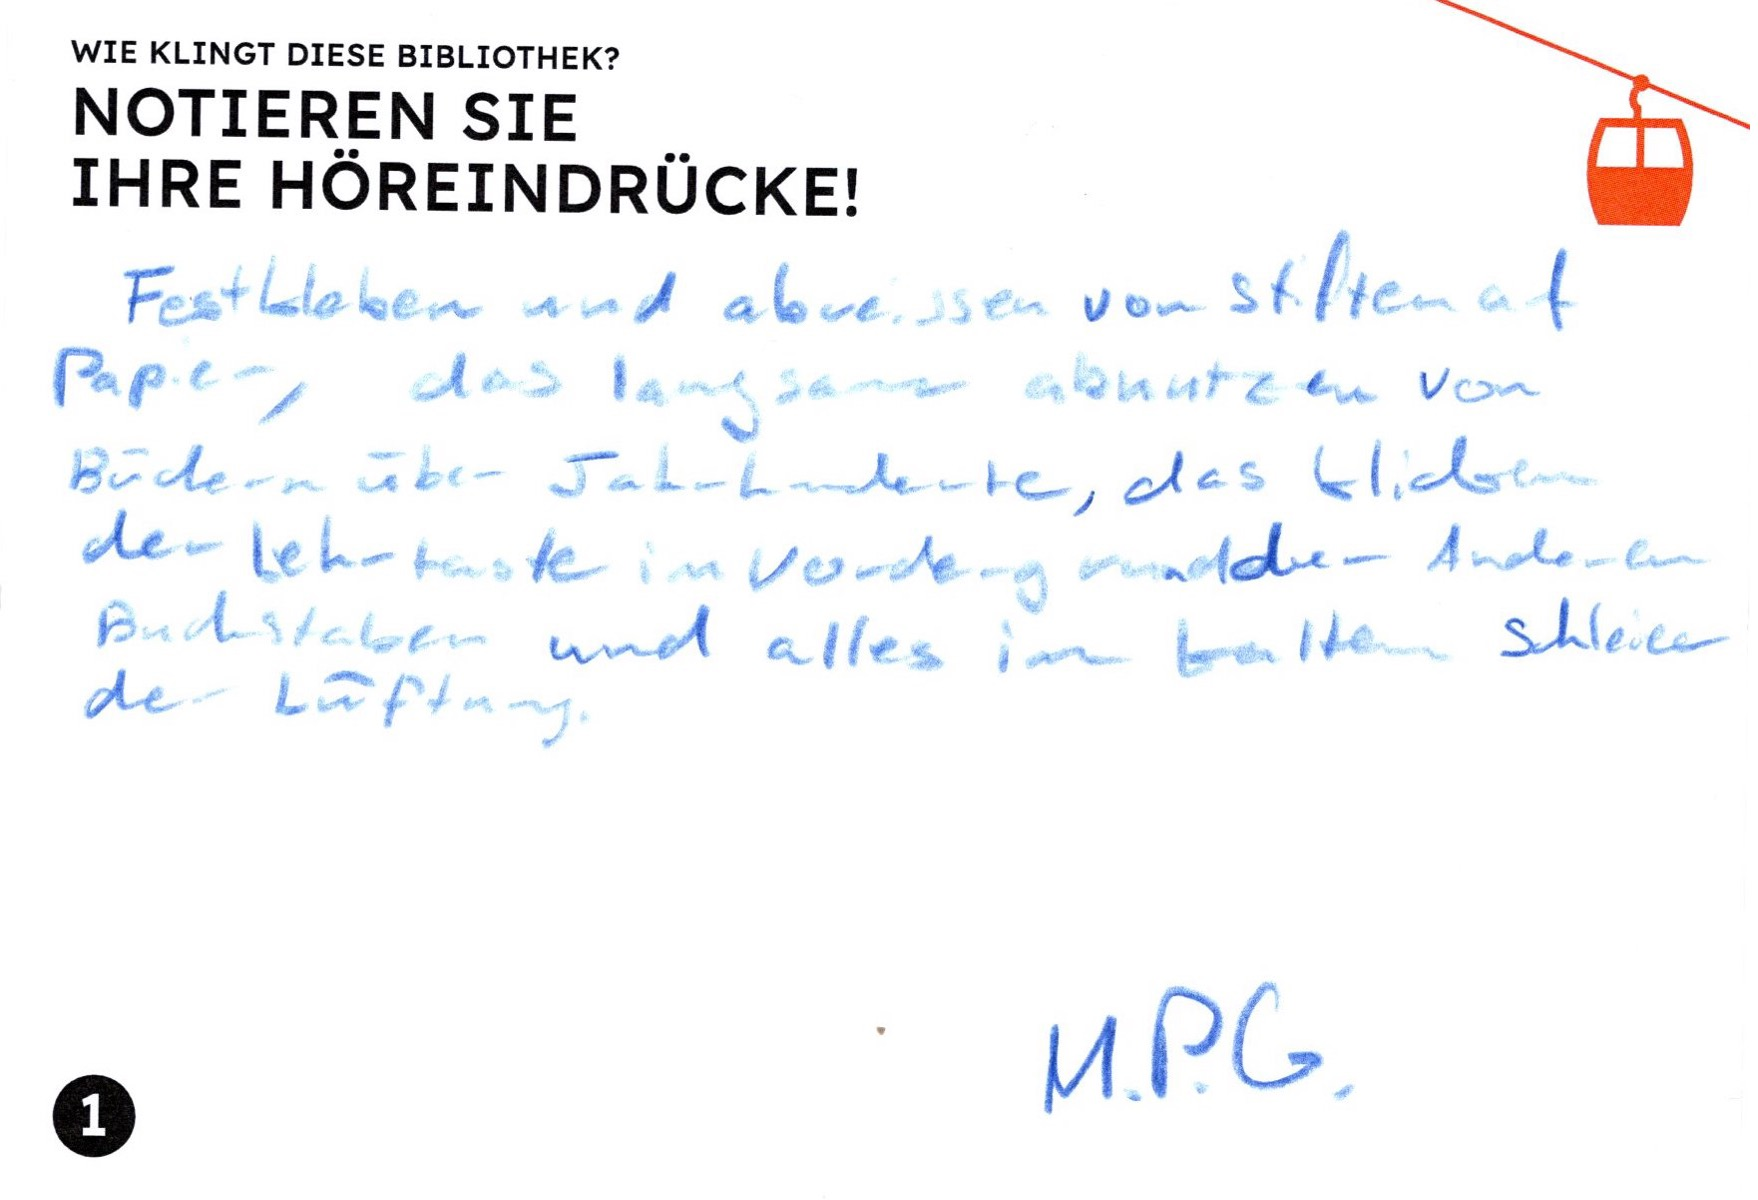
\includegraphics[width=\textwidth]{img/Abb9.jpg}
    \end{minipage}
    
    \caption{Abbildung 6-9: Auswahl beschrifteter Postkarten mit Höreindrücken vom Klang der Vera Oeri Bibliothek. Ein häufiges Thema war die Lüftung und sich nicht ruhig verhaltende Gäste.}
\end{figure}



\hypertarget{huxf6rachse-2}{%
\subsection{3. Hörachse}\label{huxf6rachse-2}}

Das Publikum konnte auf diesen Postkarten auch eigene Hörerinnerungen
festhalten, wobei einige Beiträge ebenfalls die Musikbibliothek
thematisierten:

\begin{figure}[h]
    \centering
    \begin{minipage}[b]{0.32\textwidth}
        \centering
        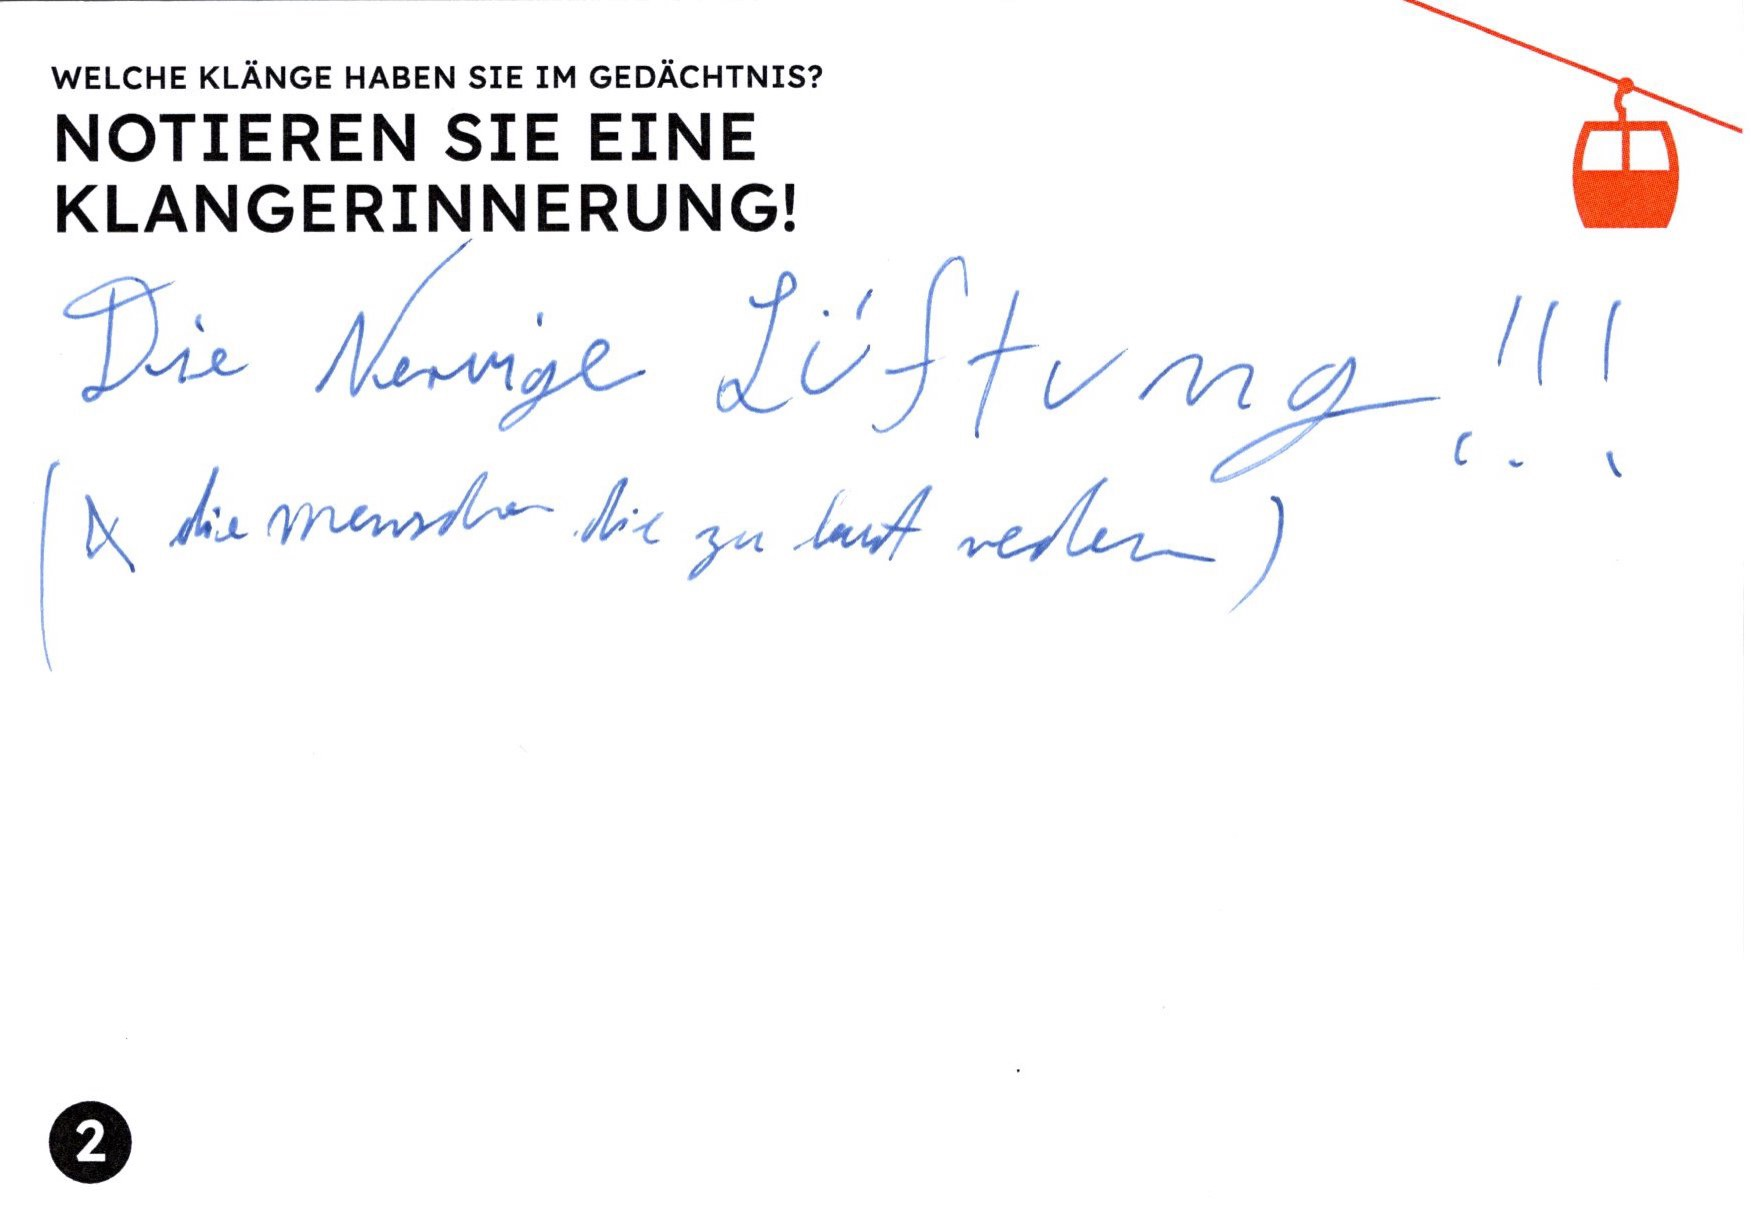
\includegraphics[width=\textwidth]{img/Abb10.jpg}
    \end{minipage}
    \begin{minipage}[b]{0.32\textwidth}
        \centering
        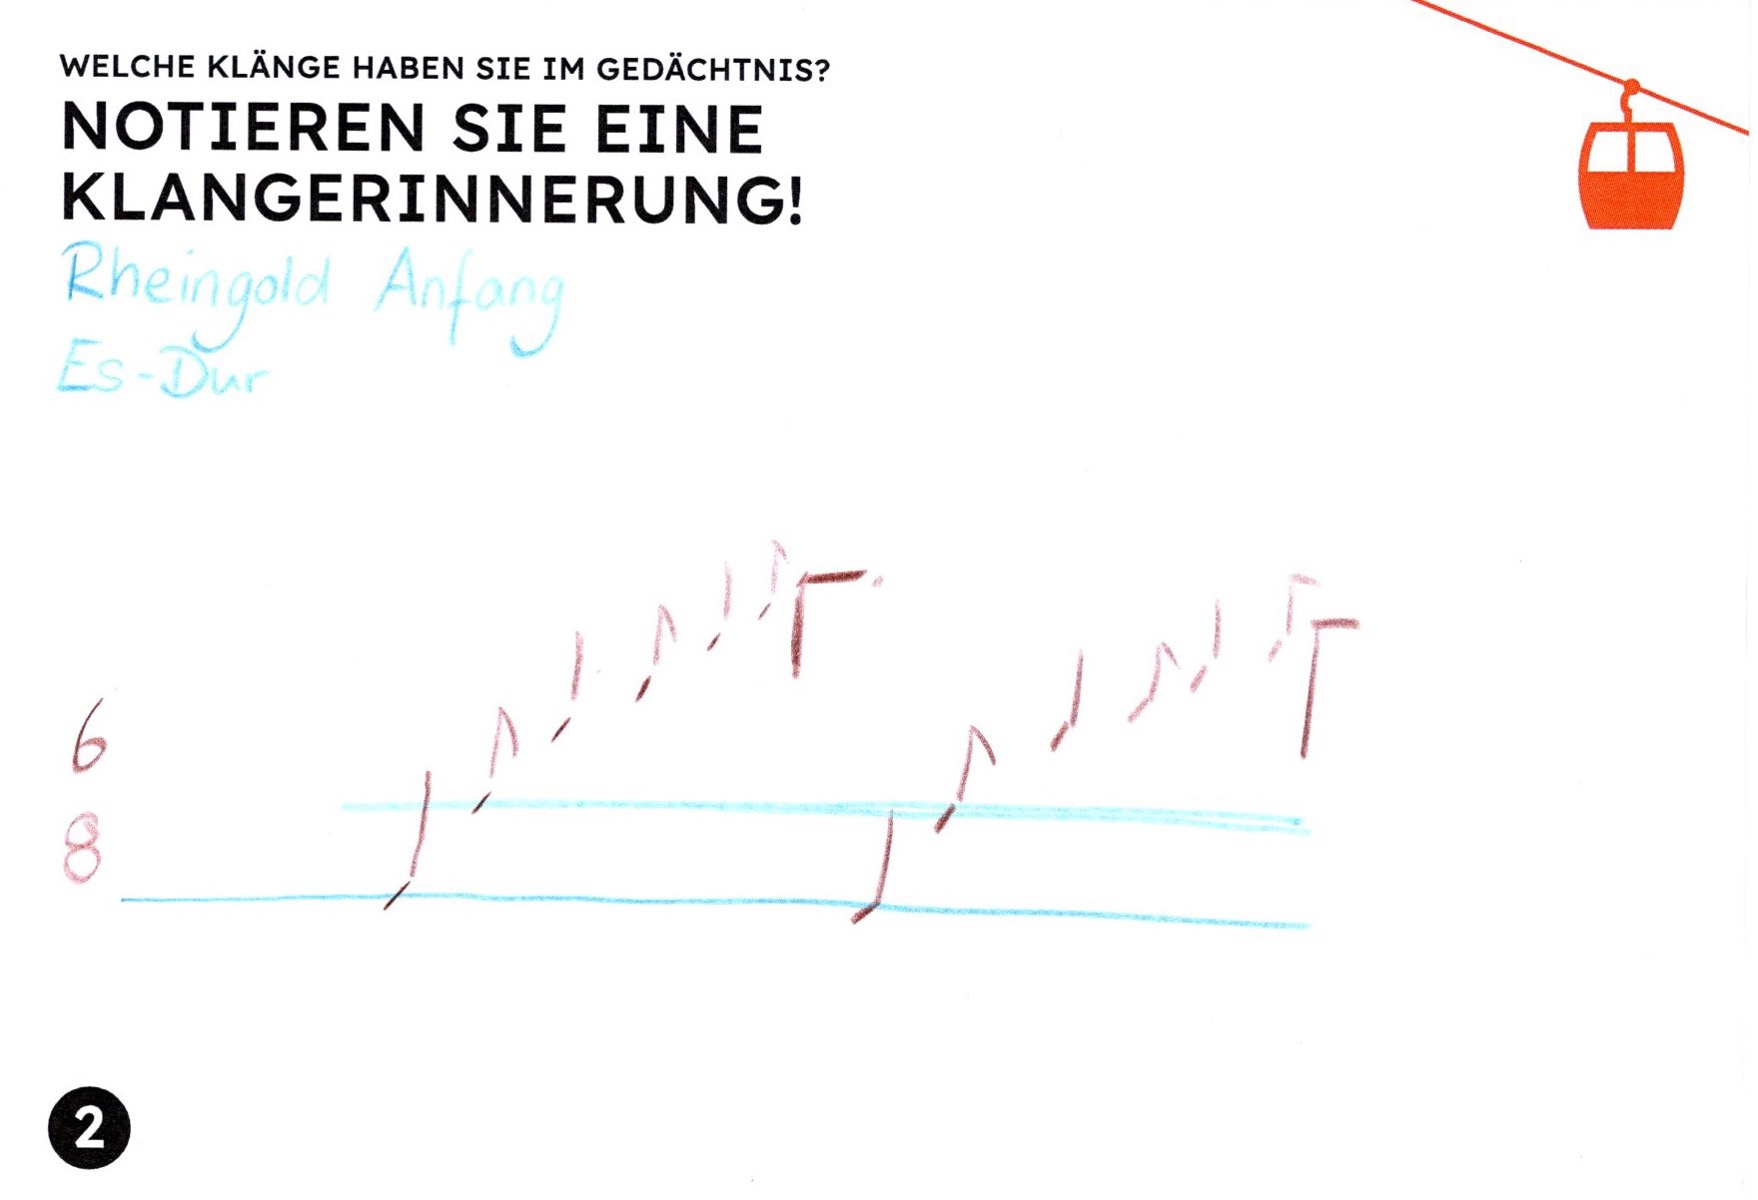
\includegraphics[width=\textwidth]{img/Abb11.jpg}
    \end{minipage}
    \begin{minipage}[b]{0.32\textwidth}
        \centering
        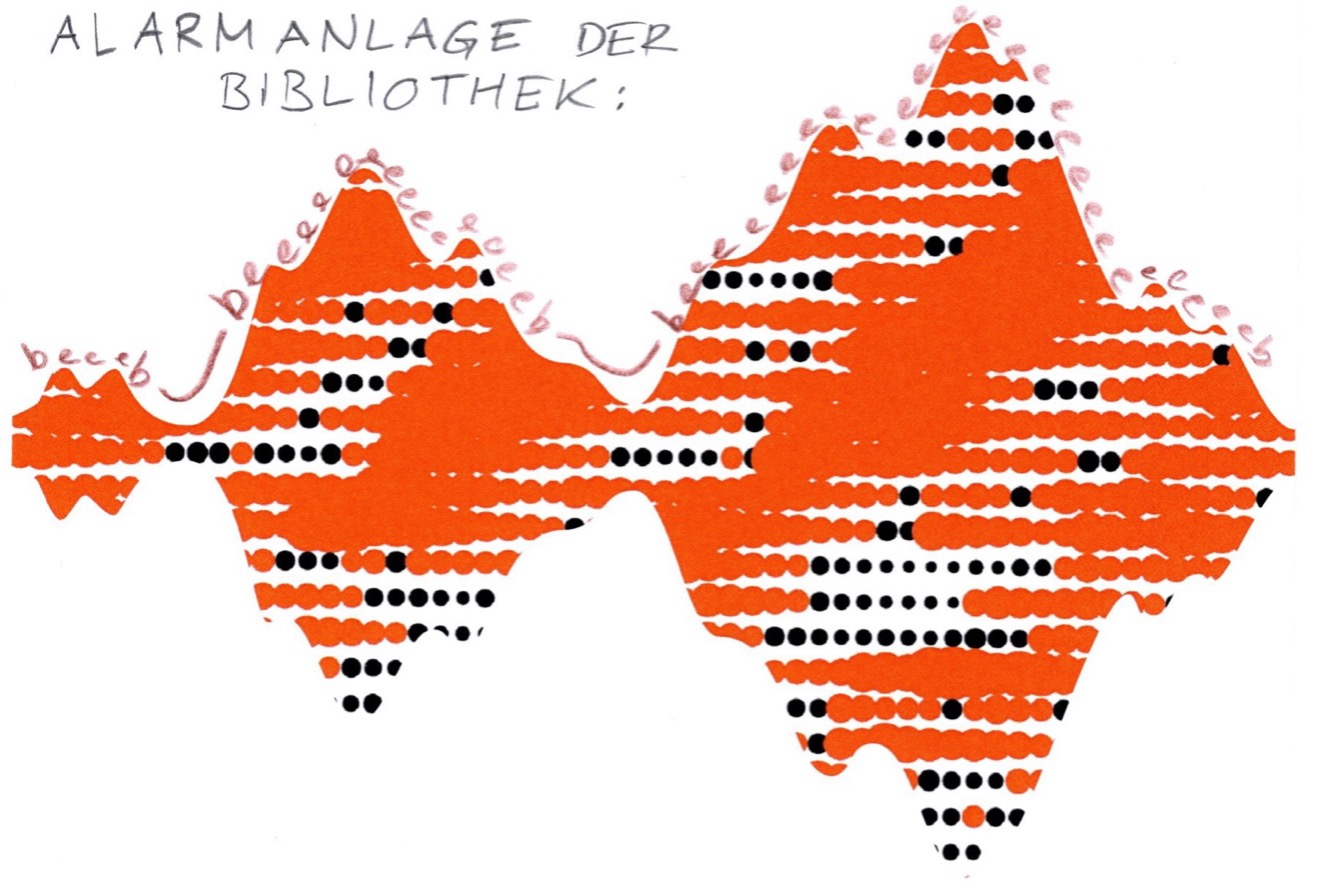
\includegraphics[width=\textwidth]{img/Abb12.jpg}
    \end{minipage}
            \caption{Abbildung 10-12: Beschriftete Postkarten mit Klangerinnerungen, Auswahl von Beispielen mit Bezug zur Musikbibliothek. Jemand hat eine Visualisierung einer Seilbahntonaufnahme kurzerhand auf den Klang der Alarmanlage der Vera Oeri Bibliothek bezogen.}
\end{figure}


Die mehrfach erwähnte Lüftung der Bibliothek, die sowohl positiv
(\enquote{Wasserfall}) als auch negativ (\enquote{nervig}) konnotiert
wurde, wurde mit Roths Forschungsmethode in die Ausstellung integriert,
indem nebst dem \enquote{Singen} von zwei Seilbahnen auch das Rauschen
eines Lüftungsrohrs der Bibliothek über Hunderte von Stunden live
gestreamt wurde.

\begin{figure}
\centering
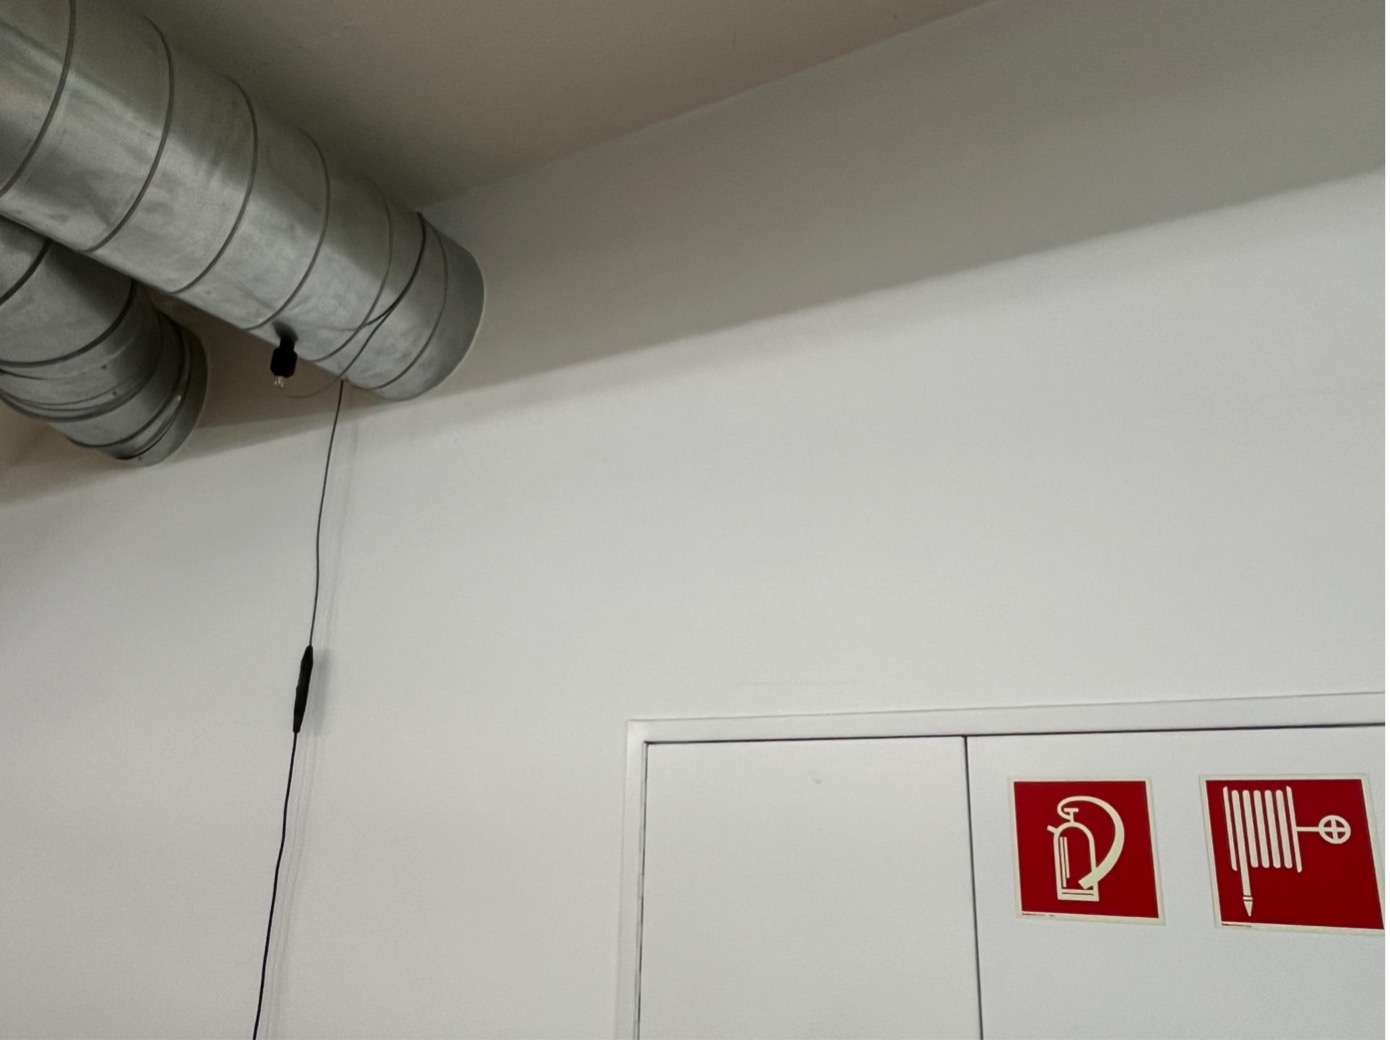
\includegraphics{img/Abb13.jpg}
\caption{Abbildung 13: Das kräftige Rauschen im Innern der Lüftungsrohre
der Vera Oeri Bibliothek wird mit einem Kontaktmikrophon aufgezeichnet
und als Livestream in die Ausstellung integriert. Als der Gitarrist
Mikael Szafirowski mit diesem Livestream musizierte, kam es zu zwei
Rückkopplungen, die in der folgenden Aufnahme dokumentiert sind (ab
Minute 7 und ab Minute 22):
\url{https://soundcloud.com/user-975110633/aircondition}; Foto: Michel
Roth.}
\end{figure}

\hypertarget{huxf6rachse-3}{%
\subsection{4. Hörachse}\label{huxf6rachse-3}}

Und schliesslich durften innere Klangvorstellungen oder kreative
Klangideen auf Postkarten festgehalten werden -- was wiederum einige
Besuchende direkt auf die Bibliothek und ihre Infrastruktur bezogen
haben:


\begin{figure}[h]
    \centering
    \begin{minipage}[b]{0.45\textwidth}
        \centering
        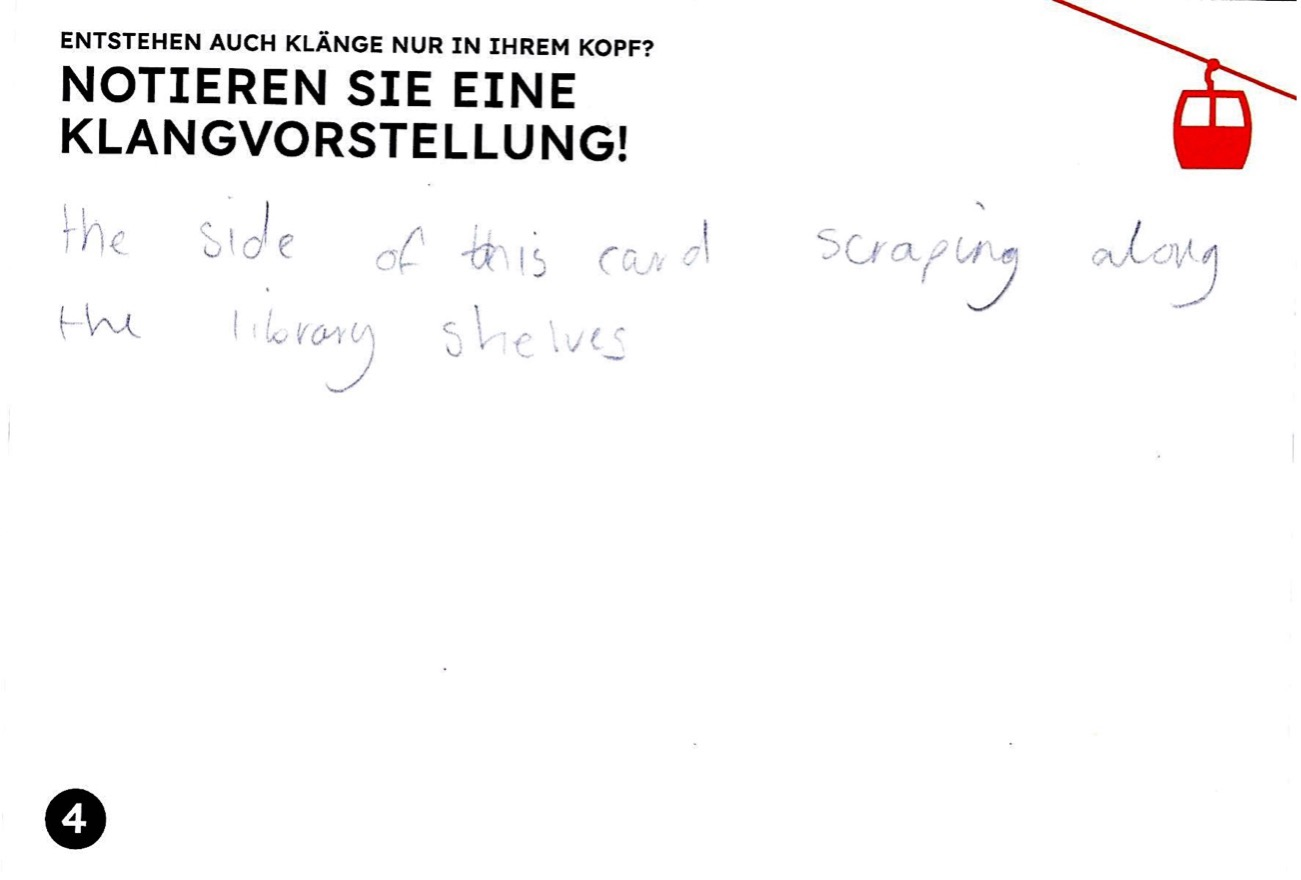
\includegraphics[width=\textwidth]{img/Abb14.jpg}
    \end{minipage}
    \begin{minipage}[b]{0.45\textwidth}
        \centering
        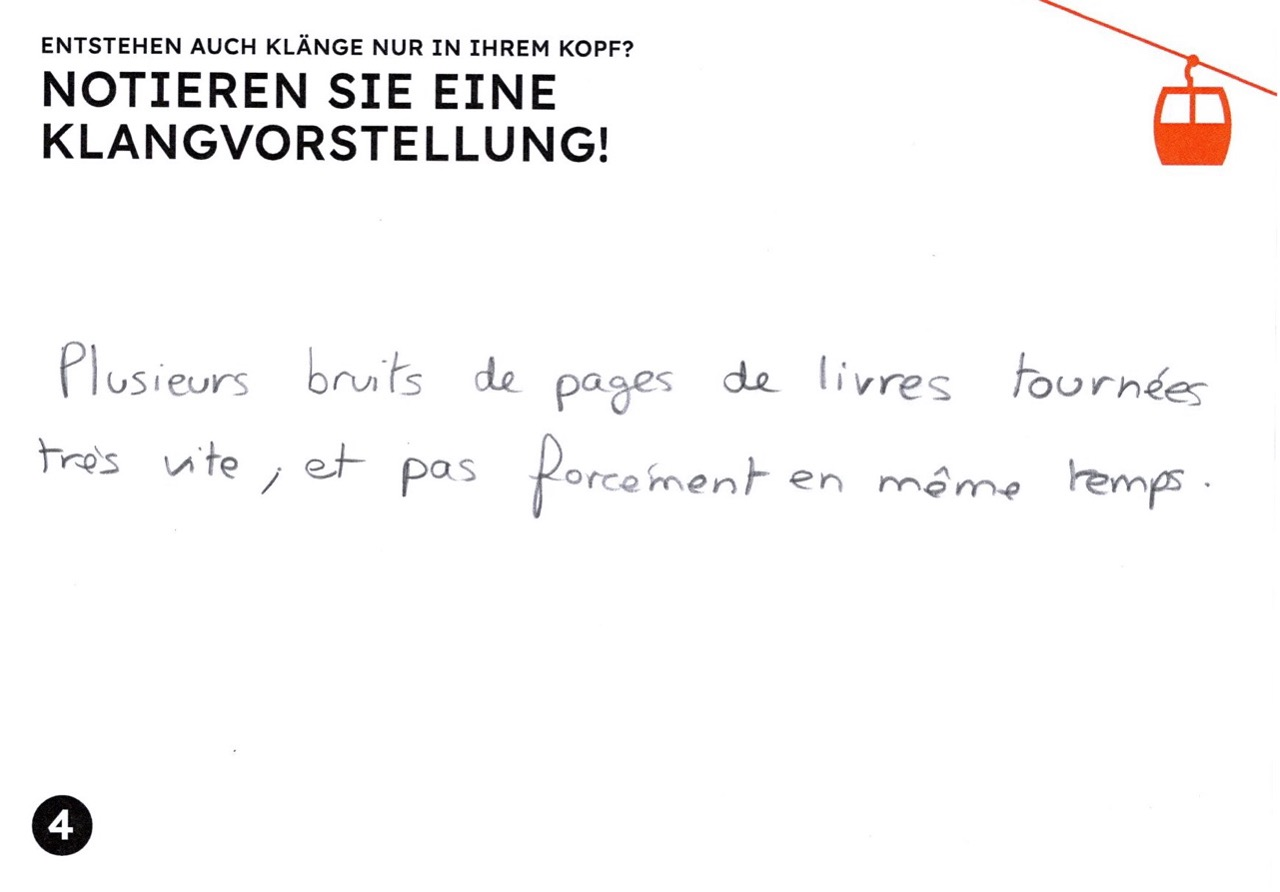
\includegraphics[width=\textwidth]{img/Abb15.jpg}
    \end{minipage}
    \caption{Abbildung 14-15: Auswahl beschrifteter Postkarten mit Klangvorstellungen: Beide Beispiele nutzen die Infrastruktur der Bibliothek, Bücher und Regale, als Klanggenerator.}
\end{figure}


Über die Ausstellungsdauer akkumulierten sich so auf den Magnettafeln
etwa 90 Beiträge von Besucher:innen der Ausstellung oder zufällig
anwesenden Nutzer:innen der Bibliothek.

\begin{figure}
\centering
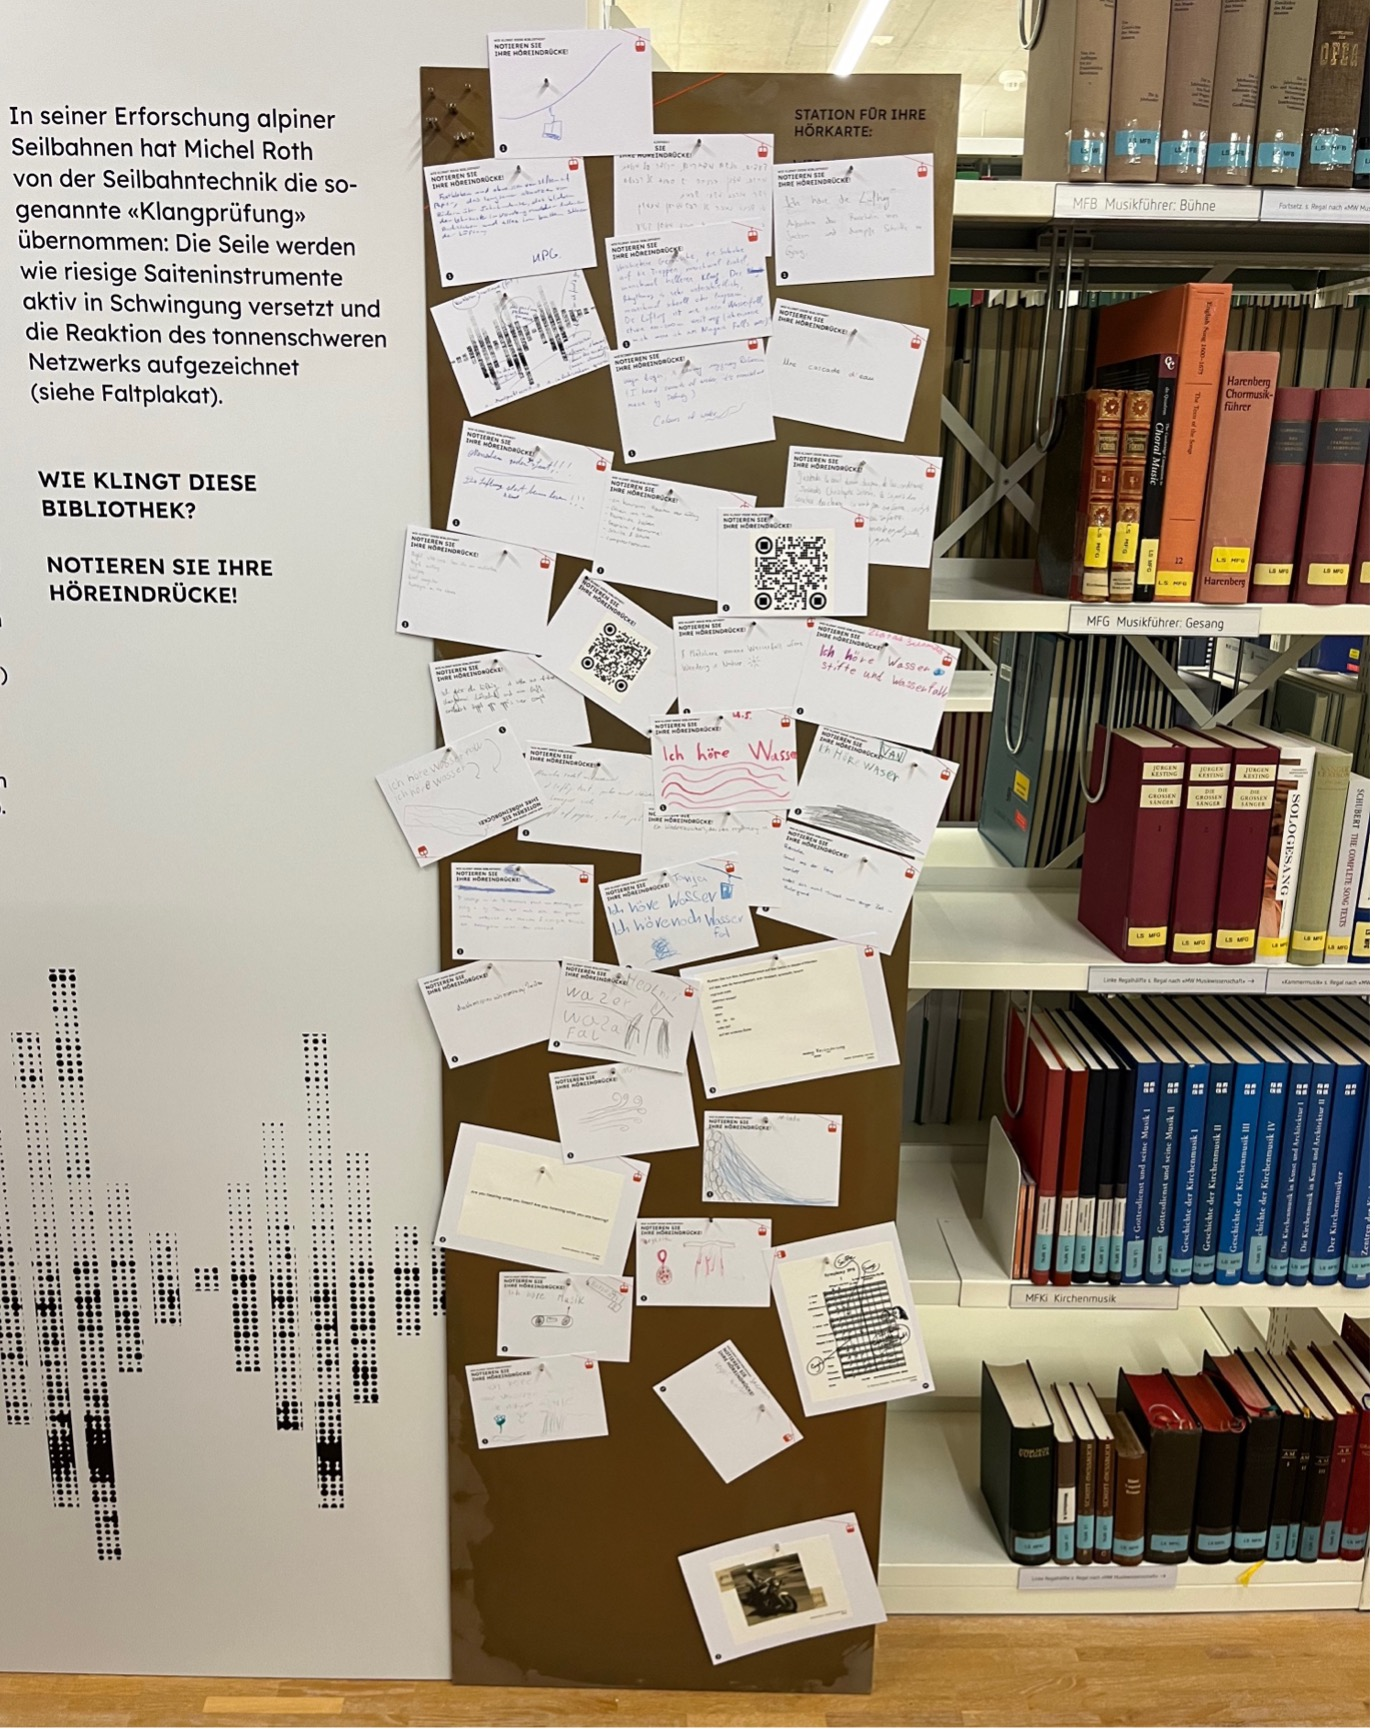
\includegraphics{img/Abb16.jpg}
\caption{Abbildung 16: Eine Magnettafel mit beschrifteten Postkarten zum
Klang der Vera Oeri Bibliothek. Foto: Michel Roth.}
\end{figure}

Ein wichtiger Bestandteil des Projekts waren konzentrierte akustische
Interventionen in die akustische Ökologie der Bibliothek: Eine immersive
Klanginstallation übertrug fühl- und hörbar Seilbahnschwingungen auf die
Metallstreben des Bibliotheksfoyers, der Ruheraum der Bibliothek wurde
an einem Tag mit wellenartigen Schwingungen des Seils einer Basler
Rheinfähre geflutet, in den Rollschränken wurden kleine Lautsprecher mit
kaum hörbaren elektronischen Summtönen versteckt, im Ausstellungsverlauf
wurden mehrere Performances oder performative Führungen in der
Bibliothek veranstaltet (siehe oben die erste Abbildung dieses
Beitrags).

\hypertarget{huxf6r-spiele}{%
\subsection{Hör-Spiele}\label{huxf6r-spiele}}

Und wie klingt eine Bibliothek mit 18 lebhaften Kindern? Wie kann man
diesen Kindern zwischen neun und zwölf Jahren vermitteln, dass nicht nur
Melodie und Rhythmus schöne Klänge sind, sondern auch alltägliche
Geräusche, die wir vielleicht gar nicht beachten, zu Musik werden
können? Als Teil der Ausstellung \emph{Singende Seile. Klingende Stadt}
fand ein mehrteiliger Workshop mit einer ukrainischen Schulklasse statt,
geleitet von der Sängerin und Musikvermittlerin Felicitas Erb zusammen
mit den Musikstudentinnen Oleksandra Katsalap und Anna Alexay und der
ukrainisch-schweizerischen Lehrerin Yelizaveta Kozlova.

Die Schüler:innen, die teilweise erst seit Kriegsausbruch in der Schweiz
wohnen, wurden zunächst durch \enquote{Hör-Spiele} sensibilisiert für
die alltäglichen Klänge ihrer Umgebung. Viele Experimente entstammten
didaktischen Medien aus dem Bestand der Vera Oeri Bibliothek. Dann haben
die Kinder ein Hörtagebuch geführt, in dem sie einen Tag lang alles
Gehörte aufgeschrieben haben. Ein Kind schrieb: \enquote{Das höre ich am
Morgen: Stille. Dann ruft meine Mutter:}Steh auf!'' Dann höre ich das
leise Knistern meines Hochbettes, wenn ich herunterstieg. Den
Wasserhahn. Die Schritte von meinen Füssen\ldots{} und so weiter\ldots''

\begin{figure}
\centering
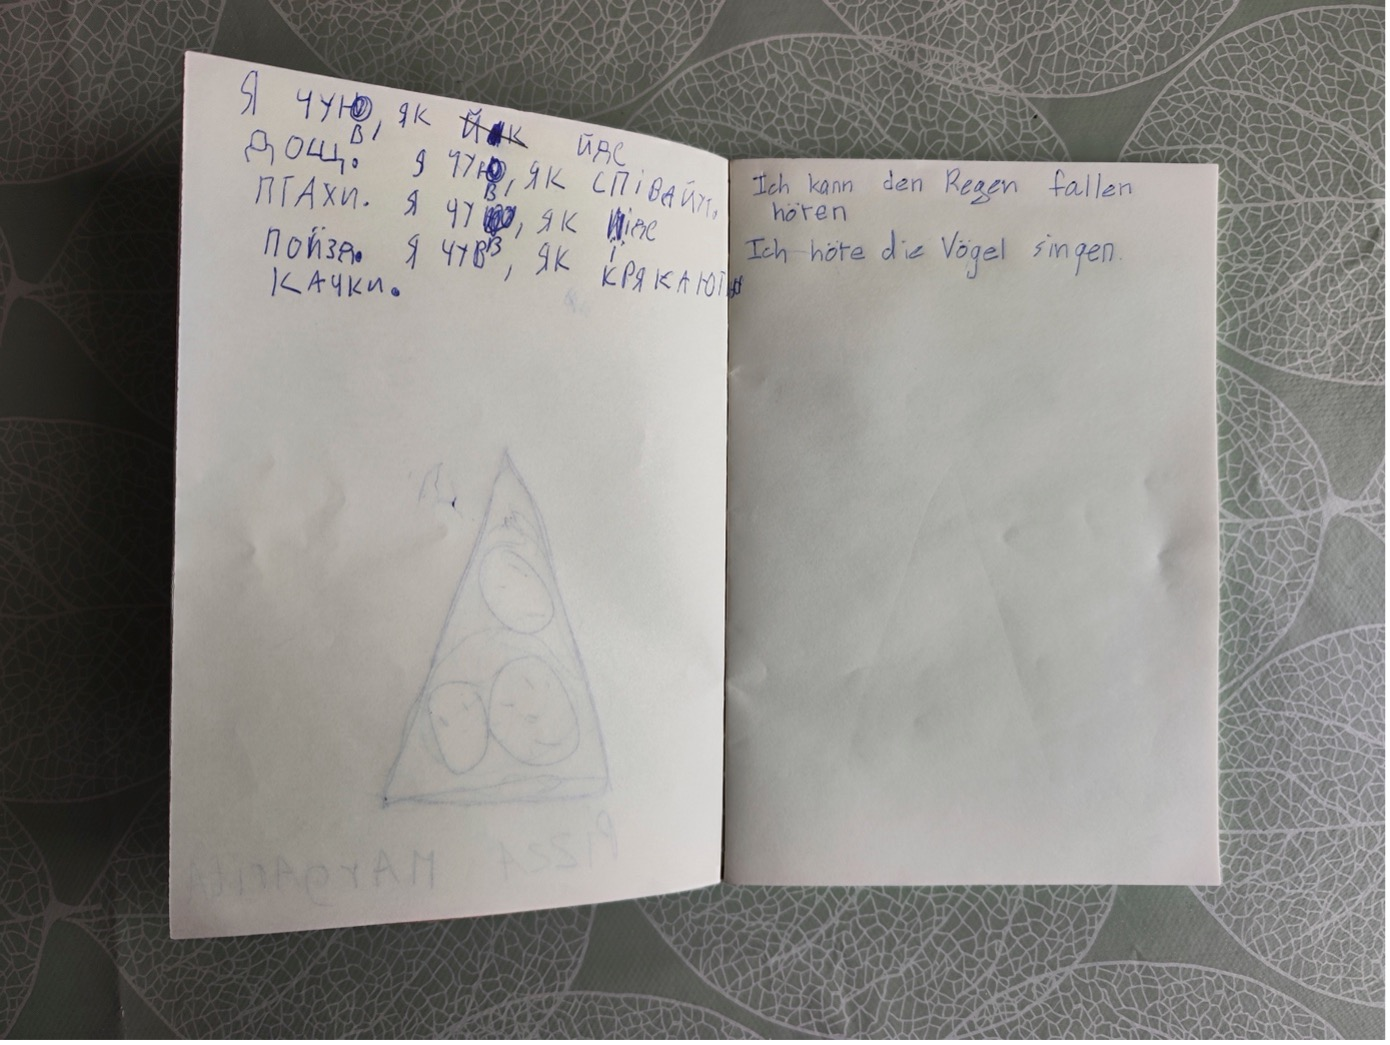
\includegraphics{img/Abb17.jpg}
\caption{Abbildung 17: Hörtagebuch Ukrainisch--Deutsch einer Schülerin der
ukrainischen Schulklasse Basel-Stadt. Foto: zvg.}
\end{figure}

\hypertarget{eigene-klangruxe4ume-komponieren}{%
\section{Eigene Klangräume
komponieren}\label{eigene-klangruxe4ume-komponieren}}

Auch die Bibliothek und die Ausstellung \emph{Singende Seile. Klingende
Stadt} wurde von den Kindern klanglich erkundet. Dazu brachte Michel
Roth spezielle Flummibälle mit, mit denen er gelegentlich Seilbahnen
künstlich zum \enquote{Singen} bringen kann. Als Klangobjekte dienten
den Kindern aber nun die Metallregale, Fensterscheiben und
Holzoberflächen der Bibliothek -- der ganze Raum wurde zum vibrierenden
Resonanzkörper. Doch selbst als die Kinder ruhig waren, bemerkten sie,
dass es in der Musikbibliothek keineswegs so leise ist, wie man vermuten
könnte: Die Lüftung tönte für viele wie ein rauschender Wasserfall.

Schliesslich konnten die Kinder eigene Kompositionserfahrungen sammeln.
In kleinen Gruppen haben sie Hörausflüge rund um die Musik-Akademie und
die Bibliothek gemacht und Klänge mit Mikrophonen aufgezeichnet:
Türenschlagen, Vogelzwitschern, Wasserrauschen, jemand übt in einem
Zimmer Klavier, Atmen, Kichern. Dabei haben die Kinder sehr verschieden
mit ihrer Klangumgebung interagiert. Die meisten waren zum ersten Mal
auf dem Campus und haben einfach die \emph{Soundscape} erforscht und
beobachtet. Andere haben aktiv etwas geändert, haben gesprochen und
sogar Rhythmen auf Objekten gespielt. Daraus sind am Computer
faszinierende Hörstücke entstanden, wie das folgende Beispiel zeigt:
\url{https://soundcloud.com/user-975110633/bohdan}

\hypertarget{klang-als-heimat}{%
\section{Klang als Heimat}\label{klang-als-heimat}}

In der Abschlusspräsentation am 24. März 2024 in der Vera Oeri
Bibliothek haben die Schüler:innen vor den Eltern und interessierten
Zuhörer:innen aus ihren Hörtagebüchern vorgelesen und ihre Kompositionen
präsentiert.

\begin{figure}
\centering
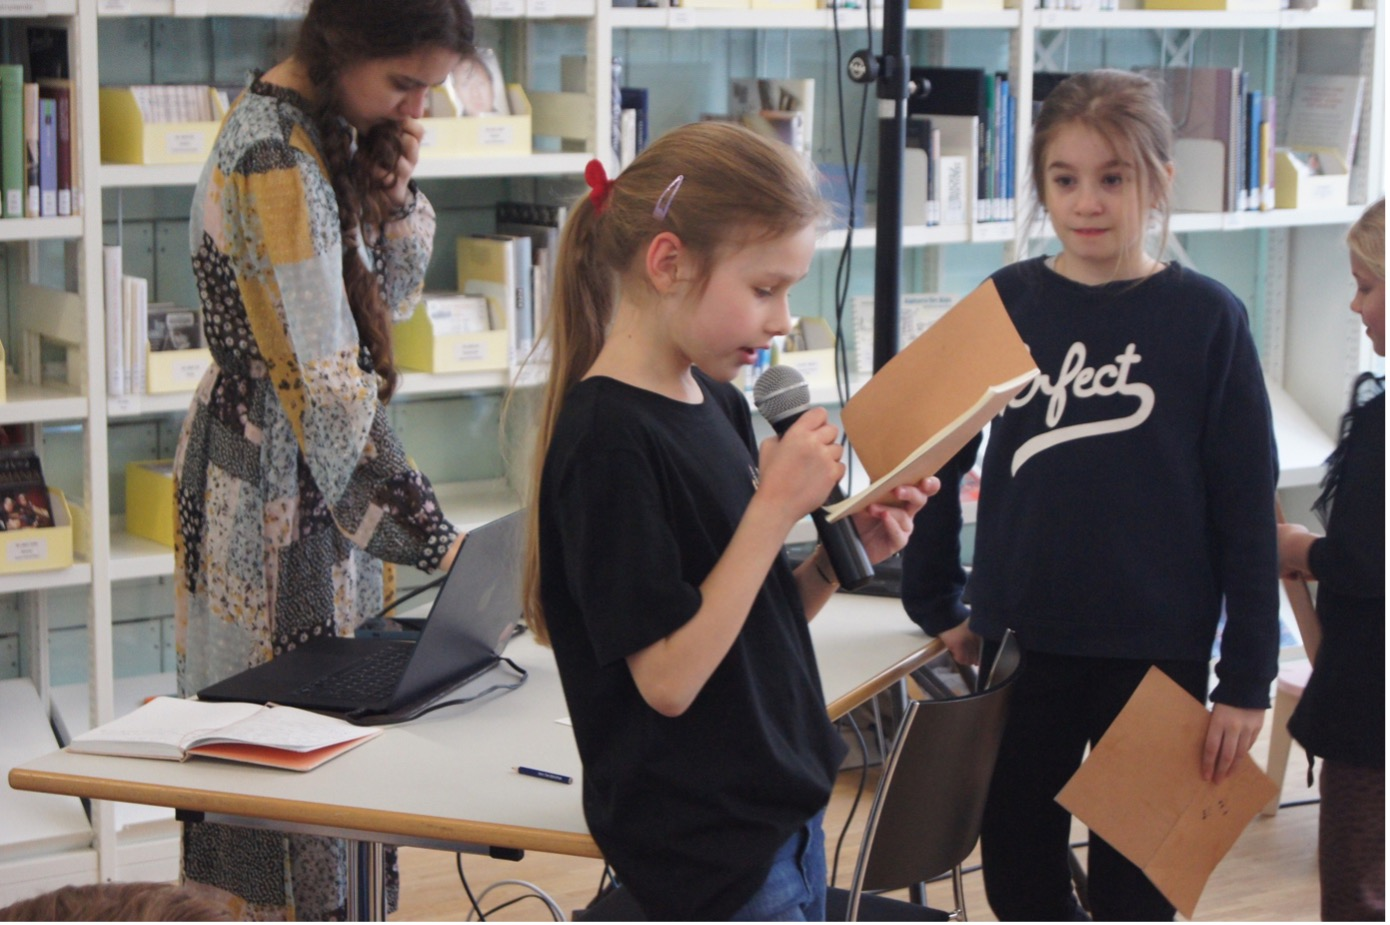
\includegraphics{img/Abb18.jpg}
\caption{Abbildung 18: Abschlussperformance der ukrainischen Schulklasse Basel-Stadt
mit Lesungen aus den Hörtagebüchern und Vorstellen der
Klangkompositionen in der \enquote{Musikbox} der Vera Oeri Bibliothek
Basel. Foto: Christoph Moor.}
\end{figure}

Es wurde deutlich, welche weitreichenden Auswirkungen eine verstärkte
Aufmerksamkeit gegenüber alltäglichen Klängen haben kann: Eine
ukrainische Lehrerin und Mutter, die die Workshops begleitete, gab nach
der Aufführung die berührende Rückmeldung, dass ihr durch das Projekt
aufgefallen sei, dass man auch mitten in der Stadt Basel die Vögel
singen höre -- wie sie es von ihrem ukrainischen Heimatort kennt.

\textbf{Dank}

Wir bedanken uns herzlich beim Team der Vera Oeri Bibliothek, namentlich
beim Leiter Thomas Nierlin, für die engagierte Unterstützung und
fachkundige Mitgestaltung dieses Projekts.

%autor
\begin{center}\rule{0.5\linewidth}{0.5pt}\end{center}

\textbf{Michel Roth} (Orcid: 0000-0002-0300-9110), geboren in Altdorf
(Uri), ist Komponist und Professor für Komposition, Musiktheorie und
Artistic Research an der Hochschule für Musik der Musik-Akademie Basel
(FHNW). Er forscht und publiziert über musikalische Anwendungen von
Spieltheorie und Kybernetik (Promotion an der Universität Basel),
Organologie der zeitgenössischen Musik und alpine Klangsoziologie
(Singende Seile'').

\url{https://www.fhnw.ch/de/personen/michel-roth}

\textbf{Felicitas Erb} ist klassische Sängerin und Musikvermittlerin,
spezialisiert auf Lied- und Konzertgesang. Für ihre CD-Einspielungen
erhielt sie zahlreiche Auszeichnungen, darunter eine Nominierung für den
Opus Klassik als Sängerin des Jahres 2023. Als Musikvermittlerin war sie
am Opernhaus Zürich tätig und arbeitet nun an ihrem Forschungsprojekt
Musikvermittlung als kreativ-kritische Praxis'' an der Hochschule für
Musik Basel.

\textbf{Anna Alexay} studiert Schulmusik II C mit Hauptfach
Musikwissenschaft in Basel. Im August 2023 hat sie Michel Roth bei
seinem Installationsprojekt Seilsender am Alpentöne-Festival in Altdorf
assistiert.

\textbf{Oleksandra Katsalap} ist eine ukrainische Musikerin. Sie
studiert Komposition und Klavier an Hochschule für Musik Basel bei
Michel Roth, Caspar Johannes Walter und Tobias Schabenberger. Ihr
Hauptinteresse liegt an die Grenze zwischen Musik und Performance.

\textbf{Oliver Rutz} studierte Komposition und Musiktheorie an der
Hochschule für Musik in Basel. Wenn er nicht in einer Musikbibliothek
sitzt, interessiert er sich für gesellschaftliche Themen im urbanen und
alpinen Raum. Oliver Rutz bildet sich derzeit weiter im journalistischen
und publizistischen Bereich.

\end{document}